%\renewcommand{\theequation}{\theenumi}
%\begin{enumerate}[label=\arabic*.,ref=\thesubsection.\theenumi]
%\numberwithin{equation}{enumi}
%
%\item Draw the circumcircle of $\triangle ABC$, where 
%
\item Verify whether 2 and 0 are zeroes of the polynomial $x^2-2x$.
\\
\solution 
The given curve 
\begin{align}
	y =\frac{1}{x-1}
\end{align}
can be expressed as 
\begin{align}
	xy - y - 1 = 0 \label{eq:solutions/1/14/eq:hyperbola}
\end{align}
Hence, we have
\begin{align}
	\vec{V} = \frac{1}{2}\myvec{0 & 1 \\ 1 & 0}, 
	\vec{u} = \frac{1}{2}\myvec{0 \\-1},
	f = -1
\end{align}
Since $\mydet{\vec{V}} < 0$, the equation \eqref{eq:solutions/1/14/eq:hyperbola} represents hyperbola.
To find the values of $\lambda_1$ and $\lambda_2$, consider the characteristic equation,
\begin{align}
	\mydet{\lambda\vec{I} - \vec{V}} &= 0\\
	\implies \mydet{\myvec{\lambda & 0\\0 & \lambda} - \myvec{0 & \frac{1}{2} \\ \frac{1}{2} & 0}} &= 0\\
	\implies \mydet{ \lambda & \frac{-1}{2} \\ \frac{-1}{2} & \lambda} &= 0\\
	\implies \lambda_1 &= \frac{1}{2} , \lambda_2 = \frac{-1}{2}
\end{align}
In addition, given the slope -1, the direction and normal vectors are given by 
\begin{align}
	\vec{m} = \myvec{1 \\ -1} \\
	\vec{n} = \myvec{ 1 \\ 1}
\end{align}
The parameters of hyperbola are as follows:
\begin{align}
	\vec{c} &= -\vec{V}^{-1}\vec{u} \\
	&= -\myvec{0 & 2\\ 2 & 0}\myvec{0 \\ -\frac{1}{2}} \\
	&= \myvec{1 \\ 0}\\
	axes &= \begin{cases}
	\sqrt{\frac{\vec{u}^T\vec{V}^{-1}\vec{u} - f}{\lambda_1}} = \sqrt{2}\\
 \sqrt{\frac{f-\vec{u}^T\vec{V}^{-1}\vec{u}}{\lambda_2}} = \sqrt{2}
\end{cases}
\end{align}
which represents the standard hyperbola equation,
\begin{align}
	\frac{x^2}{2} - \frac{x^2}{2} = 1
\end{align}
The points of contact are given by 
\begin{align}
  \tiny{K} &=\pm \sqrt{\frac{\vec{u}^T\vec{V}^{-1}\vec{u} - f}{\vec{n}^T\vec{V}^{-1}\vec{n}}}
  = \pm \frac{1}{2}\\
  \vec{q} &= \vec{V}^{-1}(k\vec{n}-\vec{u})\\
  \vec{q_1} &= \myvec{0 & 2\\2 & 0} \sbrak{\frac{1}{2}\myvec{1 \\ 1} - \myvec{0\\ \frac{-1}{2}}}\\
  &= \myvec{2 \\ 1}\\
  \vec{q_2} &= \myvec{0 & 2\\2 & 0} \sbrak{\frac{-1}{2}\myvec{1 \\ 1} - \myvec{0\\ \frac{-1}{2}}}\\
  &= \myvec{0 \\ -1}
\end{align} 
$\therefore$ The tangents are given by
\begin{align}
	\myvec{1 & 1} \brak{\vec{x} - \myvec{2 \\ 1}} = 0 \\
	\myvec{1 & 1} \brak{\vec{x} - \myvec{0 \\ -1}} = 0
\end{align}
The desired equations of all lines having slope -1 that are tangents to the curve $\frac{1}{x-1}, x \neq 1$ are given by
\begin{align}
	\myvec{1 & 1}\vec{x} &= 3 \\
	\myvec{1 & 1}\vec{x} &= -1 
\end{align}
The above results are verified in the following figure.
\begin{figure}[h!] \label{eq:solutions/1/14/fig:tangents}
	\centering
	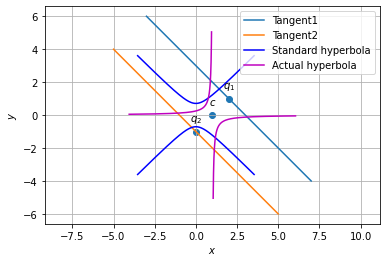
\includegraphics[width=\columnwidth]{./solutions/1/14/graph7.png}
	\caption{The standard and actual hyperbola.}
\end{figure}

\item Find $p(0)$, $p(1)$ and $p(2)$ for each of the following polynomials: 
\begin{enumerate}
\item $p(y) = y^2$. 
\item $p(x) = (x – 1) (x + 1)$.
\end{enumerate}
\solution 
The given curve 
\begin{align}
	y =\frac{1}{x-1}
\end{align}
can be expressed as 
\begin{align}
	xy - y - 1 = 0 \label{eq:solutions/1/14/eq:hyperbola}
\end{align}
Hence, we have
\begin{align}
	\vec{V} = \frac{1}{2}\myvec{0 & 1 \\ 1 & 0}, 
	\vec{u} = \frac{1}{2}\myvec{0 \\-1},
	f = -1
\end{align}
Since $\mydet{\vec{V}} < 0$, the equation \eqref{eq:solutions/1/14/eq:hyperbola} represents hyperbola.
To find the values of $\lambda_1$ and $\lambda_2$, consider the characteristic equation,
\begin{align}
	\mydet{\lambda\vec{I} - \vec{V}} &= 0\\
	\implies \mydet{\myvec{\lambda & 0\\0 & \lambda} - \myvec{0 & \frac{1}{2} \\ \frac{1}{2} & 0}} &= 0\\
	\implies \mydet{ \lambda & \frac{-1}{2} \\ \frac{-1}{2} & \lambda} &= 0\\
	\implies \lambda_1 &= \frac{1}{2} , \lambda_2 = \frac{-1}{2}
\end{align}
In addition, given the slope -1, the direction and normal vectors are given by 
\begin{align}
	\vec{m} = \myvec{1 \\ -1} \\
	\vec{n} = \myvec{ 1 \\ 1}
\end{align}
The parameters of hyperbola are as follows:
\begin{align}
	\vec{c} &= -\vec{V}^{-1}\vec{u} \\
	&= -\myvec{0 & 2\\ 2 & 0}\myvec{0 \\ -\frac{1}{2}} \\
	&= \myvec{1 \\ 0}\\
	axes &= \begin{cases}
	\sqrt{\frac{\vec{u}^T\vec{V}^{-1}\vec{u} - f}{\lambda_1}} = \sqrt{2}\\
 \sqrt{\frac{f-\vec{u}^T\vec{V}^{-1}\vec{u}}{\lambda_2}} = \sqrt{2}
\end{cases}
\end{align}
which represents the standard hyperbola equation,
\begin{align}
	\frac{x^2}{2} - \frac{x^2}{2} = 1
\end{align}
The points of contact are given by 
\begin{align}
  \tiny{K} &=\pm \sqrt{\frac{\vec{u}^T\vec{V}^{-1}\vec{u} - f}{\vec{n}^T\vec{V}^{-1}\vec{n}}}
  = \pm \frac{1}{2}\\
  \vec{q} &= \vec{V}^{-1}(k\vec{n}-\vec{u})\\
  \vec{q_1} &= \myvec{0 & 2\\2 & 0} \sbrak{\frac{1}{2}\myvec{1 \\ 1} - \myvec{0\\ \frac{-1}{2}}}\\
  &= \myvec{2 \\ 1}\\
  \vec{q_2} &= \myvec{0 & 2\\2 & 0} \sbrak{\frac{-1}{2}\myvec{1 \\ 1} - \myvec{0\\ \frac{-1}{2}}}\\
  &= \myvec{0 \\ -1}
\end{align} 
$\therefore$ The tangents are given by
\begin{align}
	\myvec{1 & 1} \brak{\vec{x} - \myvec{2 \\ 1}} = 0 \\
	\myvec{1 & 1} \brak{\vec{x} - \myvec{0 \\ -1}} = 0
\end{align}
The desired equations of all lines having slope -1 that are tangents to the curve $\frac{1}{x-1}, x \neq 1$ are given by
\begin{align}
	\myvec{1 & 1}\vec{x} &= 3 \\
	\myvec{1 & 1}\vec{x} &= -1 
\end{align}
The above results are verified in the following figure.
\begin{figure}[h!] \label{eq:solutions/1/14/fig:tangents}
	\centering
	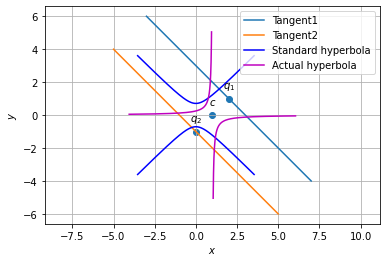
\includegraphics[width=\columnwidth]{./solutions/1/14/graph7.png}
	\caption{The standard and actual hyperbola.}
\end{figure}

\item Find the roots of the quadratic equation $6x^2– x – 2 = 0.$
\\
\solution 
	
The vector form of 
\begin{align}
y = 6x^2-x-2 
\end{align}
is
\begin{align}
	\vec{x}^T\myvec{6&0\\0&0}\vec{x}  + \myvec{-1&-1}\vec{x} -2 = 0
	\end{align}
	Thus, 
	\begin{align}
	y = 0 \quad \implies 6x^2-x-2 &= 0
	\\
	\brak{x+\frac{1}{2}}\brak{x-\frac{2}{3}} &= 0
	\\
	x = \frac{-1}{2},\frac{2}{3}&
	\end{align}
	The following python code computes roots of the quadratic equation represented in Fig. \ref{fig:5.1.5_qnineteen}.
	\begin{lstlisting}
	./solutions/5/codes/conics/q19.py
	\end{lstlisting}
	\begin{figure}[!ht]
	\centering
	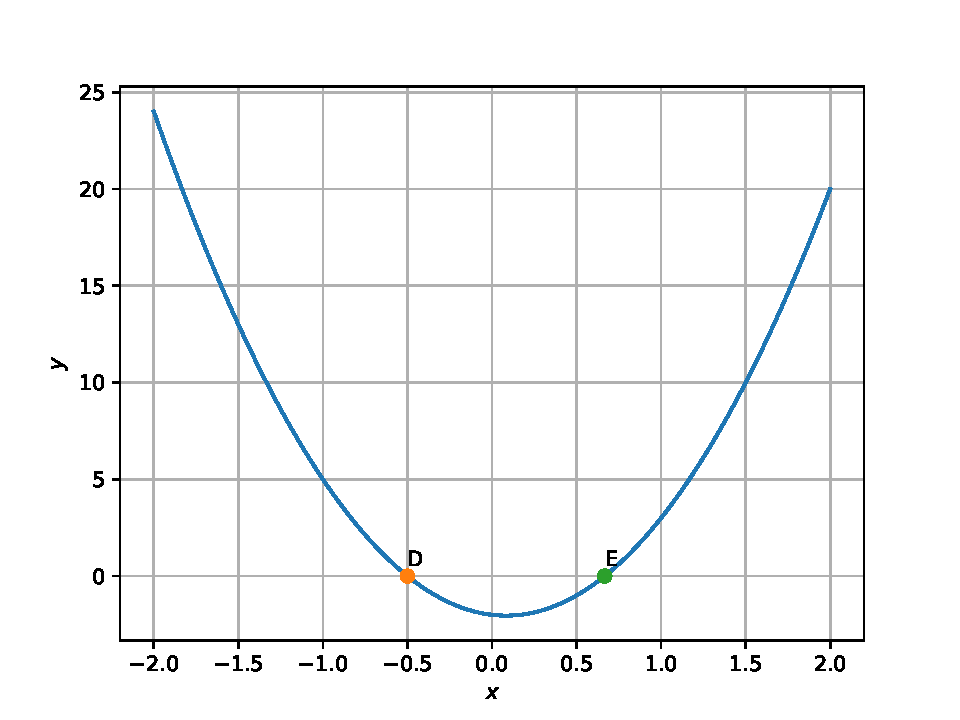
\includegraphics[width=\columnwidth]{./solutions/5/figs/conics/q19.eps}
	\caption{}
	\label{fig:5.1.5_qnineteen}	
	\end{figure}
	
	

\item Find the roots of the quadratic equation $3x^2 -2 \sqrt{6}x+ 2 = 0$.
\\
\solution 
The given curve 
\begin{align}
	y =\frac{1}{x-1}
\end{align}
can be expressed as 
\begin{align}
	xy - y - 1 = 0 \label{eq:solutions/1/14/eq:hyperbola}
\end{align}
Hence, we have
\begin{align}
	\vec{V} = \frac{1}{2}\myvec{0 & 1 \\ 1 & 0}, 
	\vec{u} = \frac{1}{2}\myvec{0 \\-1},
	f = -1
\end{align}
Since $\mydet{\vec{V}} < 0$, the equation \eqref{eq:solutions/1/14/eq:hyperbola} represents hyperbola.
To find the values of $\lambda_1$ and $\lambda_2$, consider the characteristic equation,
\begin{align}
	\mydet{\lambda\vec{I} - \vec{V}} &= 0\\
	\implies \mydet{\myvec{\lambda & 0\\0 & \lambda} - \myvec{0 & \frac{1}{2} \\ \frac{1}{2} & 0}} &= 0\\
	\implies \mydet{ \lambda & \frac{-1}{2} \\ \frac{-1}{2} & \lambda} &= 0\\
	\implies \lambda_1 &= \frac{1}{2} , \lambda_2 = \frac{-1}{2}
\end{align}
In addition, given the slope -1, the direction and normal vectors are given by 
\begin{align}
	\vec{m} = \myvec{1 \\ -1} \\
	\vec{n} = \myvec{ 1 \\ 1}
\end{align}
The parameters of hyperbola are as follows:
\begin{align}
	\vec{c} &= -\vec{V}^{-1}\vec{u} \\
	&= -\myvec{0 & 2\\ 2 & 0}\myvec{0 \\ -\frac{1}{2}} \\
	&= \myvec{1 \\ 0}\\
	axes &= \begin{cases}
	\sqrt{\frac{\vec{u}^T\vec{V}^{-1}\vec{u} - f}{\lambda_1}} = \sqrt{2}\\
 \sqrt{\frac{f-\vec{u}^T\vec{V}^{-1}\vec{u}}{\lambda_2}} = \sqrt{2}
\end{cases}
\end{align}
which represents the standard hyperbola equation,
\begin{align}
	\frac{x^2}{2} - \frac{x^2}{2} = 1
\end{align}
The points of contact are given by 
\begin{align}
  \tiny{K} &=\pm \sqrt{\frac{\vec{u}^T\vec{V}^{-1}\vec{u} - f}{\vec{n}^T\vec{V}^{-1}\vec{n}}}
  = \pm \frac{1}{2}\\
  \vec{q} &= \vec{V}^{-1}(k\vec{n}-\vec{u})\\
  \vec{q_1} &= \myvec{0 & 2\\2 & 0} \sbrak{\frac{1}{2}\myvec{1 \\ 1} - \myvec{0\\ \frac{-1}{2}}}\\
  &= \myvec{2 \\ 1}\\
  \vec{q_2} &= \myvec{0 & 2\\2 & 0} \sbrak{\frac{-1}{2}\myvec{1 \\ 1} - \myvec{0\\ \frac{-1}{2}}}\\
  &= \myvec{0 \\ -1}
\end{align} 
$\therefore$ The tangents are given by
\begin{align}
	\myvec{1 & 1} \brak{\vec{x} - \myvec{2 \\ 1}} = 0 \\
	\myvec{1 & 1} \brak{\vec{x} - \myvec{0 \\ -1}} = 0
\end{align}
The desired equations of all lines having slope -1 that are tangents to the curve $\frac{1}{x-1}, x \neq 1$ are given by
\begin{align}
	\myvec{1 & 1}\vec{x} &= 3 \\
	\myvec{1 & 1}\vec{x} &= -1 
\end{align}
The above results are verified in the following figure.
\begin{figure}[h!] \label{eq:solutions/1/14/fig:tangents}
	\centering
	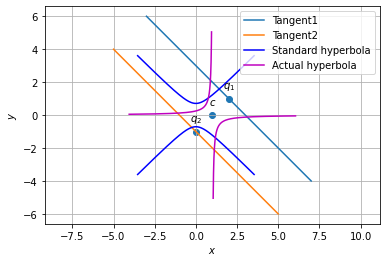
\includegraphics[width=\columnwidth]{./solutions/1/14/graph7.png}
	\caption{The standard and actual hyperbola.}
\end{figure}

\item Verify whether the following are zeroes of the polynomial, indicated against them. 
%\item p(x) = 3x + 1, x =
\begin{enumerate}

\item $ p(x) = x^2-1, x = 1, -1$
\item $ p(x) = \brak{x+1} \brak{x-2}, x = -1,2$
\item $ p(x) = x^2, x = 0$.
\item $ p(x) = 3x^2-1, x = -\frac{1}{\sqrt{3}}, \frac{2}{\sqrt{3}}$.
\end{enumerate}
\solution 
The given curve 
\begin{align}
	y =\frac{1}{x-1}
\end{align}
can be expressed as 
\begin{align}
	xy - y - 1 = 0 \label{eq:solutions/1/14/eq:hyperbola}
\end{align}
Hence, we have
\begin{align}
	\vec{V} = \frac{1}{2}\myvec{0 & 1 \\ 1 & 0}, 
	\vec{u} = \frac{1}{2}\myvec{0 \\-1},
	f = -1
\end{align}
Since $\mydet{\vec{V}} < 0$, the equation \eqref{eq:solutions/1/14/eq:hyperbola} represents hyperbola.
To find the values of $\lambda_1$ and $\lambda_2$, consider the characteristic equation,
\begin{align}
	\mydet{\lambda\vec{I} - \vec{V}} &= 0\\
	\implies \mydet{\myvec{\lambda & 0\\0 & \lambda} - \myvec{0 & \frac{1}{2} \\ \frac{1}{2} & 0}} &= 0\\
	\implies \mydet{ \lambda & \frac{-1}{2} \\ \frac{-1}{2} & \lambda} &= 0\\
	\implies \lambda_1 &= \frac{1}{2} , \lambda_2 = \frac{-1}{2}
\end{align}
In addition, given the slope -1, the direction and normal vectors are given by 
\begin{align}
	\vec{m} = \myvec{1 \\ -1} \\
	\vec{n} = \myvec{ 1 \\ 1}
\end{align}
The parameters of hyperbola are as follows:
\begin{align}
	\vec{c} &= -\vec{V}^{-1}\vec{u} \\
	&= -\myvec{0 & 2\\ 2 & 0}\myvec{0 \\ -\frac{1}{2}} \\
	&= \myvec{1 \\ 0}\\
	axes &= \begin{cases}
	\sqrt{\frac{\vec{u}^T\vec{V}^{-1}\vec{u} - f}{\lambda_1}} = \sqrt{2}\\
 \sqrt{\frac{f-\vec{u}^T\vec{V}^{-1}\vec{u}}{\lambda_2}} = \sqrt{2}
\end{cases}
\end{align}
which represents the standard hyperbola equation,
\begin{align}
	\frac{x^2}{2} - \frac{x^2}{2} = 1
\end{align}
The points of contact are given by 
\begin{align}
  \tiny{K} &=\pm \sqrt{\frac{\vec{u}^T\vec{V}^{-1}\vec{u} - f}{\vec{n}^T\vec{V}^{-1}\vec{n}}}
  = \pm \frac{1}{2}\\
  \vec{q} &= \vec{V}^{-1}(k\vec{n}-\vec{u})\\
  \vec{q_1} &= \myvec{0 & 2\\2 & 0} \sbrak{\frac{1}{2}\myvec{1 \\ 1} - \myvec{0\\ \frac{-1}{2}}}\\
  &= \myvec{2 \\ 1}\\
  \vec{q_2} &= \myvec{0 & 2\\2 & 0} \sbrak{\frac{-1}{2}\myvec{1 \\ 1} - \myvec{0\\ \frac{-1}{2}}}\\
  &= \myvec{0 \\ -1}
\end{align} 
$\therefore$ The tangents are given by
\begin{align}
	\myvec{1 & 1} \brak{\vec{x} - \myvec{2 \\ 1}} = 0 \\
	\myvec{1 & 1} \brak{\vec{x} - \myvec{0 \\ -1}} = 0
\end{align}
The desired equations of all lines having slope -1 that are tangents to the curve $\frac{1}{x-1}, x \neq 1$ are given by
\begin{align}
	\myvec{1 & 1}\vec{x} &= 3 \\
	\myvec{1 & 1}\vec{x} &= -1 
\end{align}
The above results are verified in the following figure.
\begin{figure}[h!] \label{eq:solutions/1/14/fig:tangents}
	\centering
	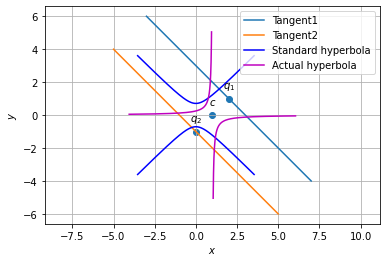
\includegraphics[width=\columnwidth]{./solutions/1/14/graph7.png}
	\caption{The standard and actual hyperbola.}
\end{figure}

\item Solve each of the following equations
\begin{enumerate}
\item 	$3x^2-4x+\frac{20}{3} = 0$
\item 	$x^2-2x+\frac{3}{2} = 0$
\item 	$27x^2-10x+1 = 0$
\item 	$21x^2-28x+10 = 0$
\end{enumerate}
%
\solution 
The given curve 
\begin{align}
	y =\frac{1}{x-1}
\end{align}
can be expressed as 
\begin{align}
	xy - y - 1 = 0 \label{eq:solutions/1/14/eq:hyperbola}
\end{align}
Hence, we have
\begin{align}
	\vec{V} = \frac{1}{2}\myvec{0 & 1 \\ 1 & 0}, 
	\vec{u} = \frac{1}{2}\myvec{0 \\-1},
	f = -1
\end{align}
Since $\mydet{\vec{V}} < 0$, the equation \eqref{eq:solutions/1/14/eq:hyperbola} represents hyperbola.
To find the values of $\lambda_1$ and $\lambda_2$, consider the characteristic equation,
\begin{align}
	\mydet{\lambda\vec{I} - \vec{V}} &= 0\\
	\implies \mydet{\myvec{\lambda & 0\\0 & \lambda} - \myvec{0 & \frac{1}{2} \\ \frac{1}{2} & 0}} &= 0\\
	\implies \mydet{ \lambda & \frac{-1}{2} \\ \frac{-1}{2} & \lambda} &= 0\\
	\implies \lambda_1 &= \frac{1}{2} , \lambda_2 = \frac{-1}{2}
\end{align}
In addition, given the slope -1, the direction and normal vectors are given by 
\begin{align}
	\vec{m} = \myvec{1 \\ -1} \\
	\vec{n} = \myvec{ 1 \\ 1}
\end{align}
The parameters of hyperbola are as follows:
\begin{align}
	\vec{c} &= -\vec{V}^{-1}\vec{u} \\
	&= -\myvec{0 & 2\\ 2 & 0}\myvec{0 \\ -\frac{1}{2}} \\
	&= \myvec{1 \\ 0}\\
	axes &= \begin{cases}
	\sqrt{\frac{\vec{u}^T\vec{V}^{-1}\vec{u} - f}{\lambda_1}} = \sqrt{2}\\
 \sqrt{\frac{f-\vec{u}^T\vec{V}^{-1}\vec{u}}{\lambda_2}} = \sqrt{2}
\end{cases}
\end{align}
which represents the standard hyperbola equation,
\begin{align}
	\frac{x^2}{2} - \frac{x^2}{2} = 1
\end{align}
The points of contact are given by 
\begin{align}
  \tiny{K} &=\pm \sqrt{\frac{\vec{u}^T\vec{V}^{-1}\vec{u} - f}{\vec{n}^T\vec{V}^{-1}\vec{n}}}
  = \pm \frac{1}{2}\\
  \vec{q} &= \vec{V}^{-1}(k\vec{n}-\vec{u})\\
  \vec{q_1} &= \myvec{0 & 2\\2 & 0} \sbrak{\frac{1}{2}\myvec{1 \\ 1} - \myvec{0\\ \frac{-1}{2}}}\\
  &= \myvec{2 \\ 1}\\
  \vec{q_2} &= \myvec{0 & 2\\2 & 0} \sbrak{\frac{-1}{2}\myvec{1 \\ 1} - \myvec{0\\ \frac{-1}{2}}}\\
  &= \myvec{0 \\ -1}
\end{align} 
$\therefore$ The tangents are given by
\begin{align}
	\myvec{1 & 1} \brak{\vec{x} - \myvec{2 \\ 1}} = 0 \\
	\myvec{1 & 1} \brak{\vec{x} - \myvec{0 \\ -1}} = 0
\end{align}
The desired equations of all lines having slope -1 that are tangents to the curve $\frac{1}{x-1}, x \neq 1$ are given by
\begin{align}
	\myvec{1 & 1}\vec{x} &= 3 \\
	\myvec{1 & 1}\vec{x} &= -1 
\end{align}
The above results are verified in the following figure.
\begin{figure}[h!] \label{eq:solutions/1/14/fig:tangents}
	\centering
	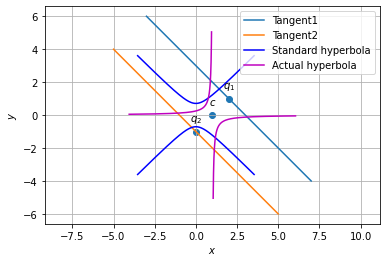
\includegraphics[width=\columnwidth]{./solutions/1/14/graph7.png}
	\caption{The standard and actual hyperbola.}
\end{figure}


%
\item  Factorise 
\begin{enumerate}
\item $12x^2 – 7x + 1 $
\item $6x^2+ 5x – 6$
\item $2x^2+ 7x + 3 $
\item $3x^2– x – 4$
\end{enumerate}
\solution 
The given curve 
\begin{align}
	y =\frac{1}{x-1}
\end{align}
can be expressed as 
\begin{align}
	xy - y - 1 = 0 \label{eq:solutions/1/14/eq:hyperbola}
\end{align}
Hence, we have
\begin{align}
	\vec{V} = \frac{1}{2}\myvec{0 & 1 \\ 1 & 0}, 
	\vec{u} = \frac{1}{2}\myvec{0 \\-1},
	f = -1
\end{align}
Since $\mydet{\vec{V}} < 0$, the equation \eqref{eq:solutions/1/14/eq:hyperbola} represents hyperbola.
To find the values of $\lambda_1$ and $\lambda_2$, consider the characteristic equation,
\begin{align}
	\mydet{\lambda\vec{I} - \vec{V}} &= 0\\
	\implies \mydet{\myvec{\lambda & 0\\0 & \lambda} - \myvec{0 & \frac{1}{2} \\ \frac{1}{2} & 0}} &= 0\\
	\implies \mydet{ \lambda & \frac{-1}{2} \\ \frac{-1}{2} & \lambda} &= 0\\
	\implies \lambda_1 &= \frac{1}{2} , \lambda_2 = \frac{-1}{2}
\end{align}
In addition, given the slope -1, the direction and normal vectors are given by 
\begin{align}
	\vec{m} = \myvec{1 \\ -1} \\
	\vec{n} = \myvec{ 1 \\ 1}
\end{align}
The parameters of hyperbola are as follows:
\begin{align}
	\vec{c} &= -\vec{V}^{-1}\vec{u} \\
	&= -\myvec{0 & 2\\ 2 & 0}\myvec{0 \\ -\frac{1}{2}} \\
	&= \myvec{1 \\ 0}\\
	axes &= \begin{cases}
	\sqrt{\frac{\vec{u}^T\vec{V}^{-1}\vec{u} - f}{\lambda_1}} = \sqrt{2}\\
 \sqrt{\frac{f-\vec{u}^T\vec{V}^{-1}\vec{u}}{\lambda_2}} = \sqrt{2}
\end{cases}
\end{align}
which represents the standard hyperbola equation,
\begin{align}
	\frac{x^2}{2} - \frac{x^2}{2} = 1
\end{align}
The points of contact are given by 
\begin{align}
  \tiny{K} &=\pm \sqrt{\frac{\vec{u}^T\vec{V}^{-1}\vec{u} - f}{\vec{n}^T\vec{V}^{-1}\vec{n}}}
  = \pm \frac{1}{2}\\
  \vec{q} &= \vec{V}^{-1}(k\vec{n}-\vec{u})\\
  \vec{q_1} &= \myvec{0 & 2\\2 & 0} \sbrak{\frac{1}{2}\myvec{1 \\ 1} - \myvec{0\\ \frac{-1}{2}}}\\
  &= \myvec{2 \\ 1}\\
  \vec{q_2} &= \myvec{0 & 2\\2 & 0} \sbrak{\frac{-1}{2}\myvec{1 \\ 1} - \myvec{0\\ \frac{-1}{2}}}\\
  &= \myvec{0 \\ -1}
\end{align} 
$\therefore$ The tangents are given by
\begin{align}
	\myvec{1 & 1} \brak{\vec{x} - \myvec{2 \\ 1}} = 0 \\
	\myvec{1 & 1} \brak{\vec{x} - \myvec{0 \\ -1}} = 0
\end{align}
The desired equations of all lines having slope -1 that are tangents to the curve $\frac{1}{x-1}, x \neq 1$ are given by
\begin{align}
	\myvec{1 & 1}\vec{x} &= 3 \\
	\myvec{1 & 1}\vec{x} &= -1 
\end{align}
The above results are verified in the following figure.
\begin{figure}[h!] \label{eq:solutions/1/14/fig:tangents}
	\centering
	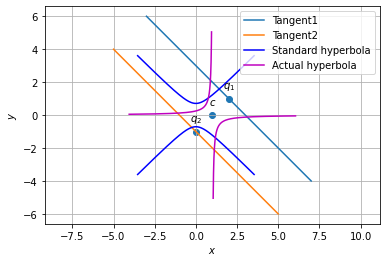
\includegraphics[width=\columnwidth]{./solutions/1/14/graph7.png}
	\caption{The standard and actual hyperbola.}
\end{figure}

\item Find the zeroes of the following quadratic polynomials and verify the relationship between the zeroes and the coefficients.
\begin{enumerate}
\item $x^2 – 2x – 8$
\item  $4u^2 + 8u$
\item $4s^2 – 4s + 1$
\item $t^2 – 15$
\item $6x^2– 3 – 7x $
\item $3x^2 – x – 4$
\end{enumerate}
\solution 
The given curve 
\begin{align}
	y =\frac{1}{x-1}
\end{align}
can be expressed as 
\begin{align}
	xy - y - 1 = 0 \label{eq:solutions/1/14/eq:hyperbola}
\end{align}
Hence, we have
\begin{align}
	\vec{V} = \frac{1}{2}\myvec{0 & 1 \\ 1 & 0}, 
	\vec{u} = \frac{1}{2}\myvec{0 \\-1},
	f = -1
\end{align}
Since $\mydet{\vec{V}} < 0$, the equation \eqref{eq:solutions/1/14/eq:hyperbola} represents hyperbola.
To find the values of $\lambda_1$ and $\lambda_2$, consider the characteristic equation,
\begin{align}
	\mydet{\lambda\vec{I} - \vec{V}} &= 0\\
	\implies \mydet{\myvec{\lambda & 0\\0 & \lambda} - \myvec{0 & \frac{1}{2} \\ \frac{1}{2} & 0}} &= 0\\
	\implies \mydet{ \lambda & \frac{-1}{2} \\ \frac{-1}{2} & \lambda} &= 0\\
	\implies \lambda_1 &= \frac{1}{2} , \lambda_2 = \frac{-1}{2}
\end{align}
In addition, given the slope -1, the direction and normal vectors are given by 
\begin{align}
	\vec{m} = \myvec{1 \\ -1} \\
	\vec{n} = \myvec{ 1 \\ 1}
\end{align}
The parameters of hyperbola are as follows:
\begin{align}
	\vec{c} &= -\vec{V}^{-1}\vec{u} \\
	&= -\myvec{0 & 2\\ 2 & 0}\myvec{0 \\ -\frac{1}{2}} \\
	&= \myvec{1 \\ 0}\\
	axes &= \begin{cases}
	\sqrt{\frac{\vec{u}^T\vec{V}^{-1}\vec{u} - f}{\lambda_1}} = \sqrt{2}\\
 \sqrt{\frac{f-\vec{u}^T\vec{V}^{-1}\vec{u}}{\lambda_2}} = \sqrt{2}
\end{cases}
\end{align}
which represents the standard hyperbola equation,
\begin{align}
	\frac{x^2}{2} - \frac{x^2}{2} = 1
\end{align}
The points of contact are given by 
\begin{align}
  \tiny{K} &=\pm \sqrt{\frac{\vec{u}^T\vec{V}^{-1}\vec{u} - f}{\vec{n}^T\vec{V}^{-1}\vec{n}}}
  = \pm \frac{1}{2}\\
  \vec{q} &= \vec{V}^{-1}(k\vec{n}-\vec{u})\\
  \vec{q_1} &= \myvec{0 & 2\\2 & 0} \sbrak{\frac{1}{2}\myvec{1 \\ 1} - \myvec{0\\ \frac{-1}{2}}}\\
  &= \myvec{2 \\ 1}\\
  \vec{q_2} &= \myvec{0 & 2\\2 & 0} \sbrak{\frac{-1}{2}\myvec{1 \\ 1} - \myvec{0\\ \frac{-1}{2}}}\\
  &= \myvec{0 \\ -1}
\end{align} 
$\therefore$ The tangents are given by
\begin{align}
	\myvec{1 & 1} \brak{\vec{x} - \myvec{2 \\ 1}} = 0 \\
	\myvec{1 & 1} \brak{\vec{x} - \myvec{0 \\ -1}} = 0
\end{align}
The desired equations of all lines having slope -1 that are tangents to the curve $\frac{1}{x-1}, x \neq 1$ are given by
\begin{align}
	\myvec{1 & 1}\vec{x} &= 3 \\
	\myvec{1 & 1}\vec{x} &= -1 
\end{align}
The above results are verified in the following figure.
\begin{figure}[h!] \label{eq:solutions/1/14/fig:tangents}
	\centering
	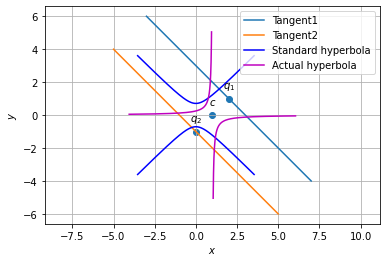
\includegraphics[width=\columnwidth]{./solutions/1/14/graph7.png}
	\caption{The standard and actual hyperbola.}
\end{figure}

\item  Find a quadratic polynomial each with the given numbers as the sum and product of its zeroes respectively.
\begin{enumerate}
\item-1 , $\frac{1}{ 4}$
\item 1, 1
\item $0, \sqrt{5}$ 
\item 4, 1
 \item $\frac{1}{4}, \frac{1}{4}$
\item  $\sqrt{2}, \frac{1}{ 3}$
\end{enumerate}
\solution 
The following python code computes roots of the quadratic equation obtained:
	\begin{lstlisting}
	./solutions/5/codes/conics/q20a.py
	./solutions/5/codes/conics/q20b.py
	./solutions/5/codes/conics/q20c.py
	./solutions/5/codes/conics/q20d.py
	./solutions/5/codes/conics/q20e.py
	./solutions/5/codes/conics/q20f.py
	\end{lstlisting}
	
	\begin{enumerate}
	
		\item -1,$\frac{1}{4}$
	\begin{figure}[!ht]
	\centering
	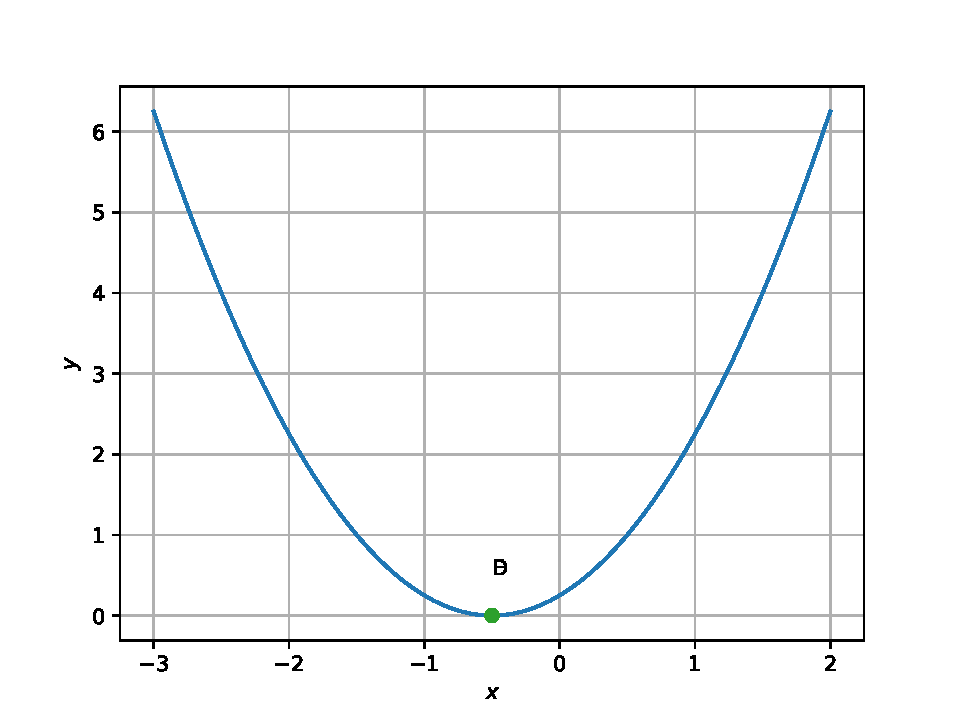
\includegraphics[width=\columnwidth]{./solutions/5/figs/conics/q20a.eps}
	\caption{}
	\label{fig:5.2.5_qtoa}	
	\end{figure}
	
		 For a general polynomial equation of degree 2,
	\begin{multline}
	p\brak{x,y} =
\\
 Ax^2 +Bxy + Cy^2 +Dx + Ey + F = 0\\
	\text{The vector form is}\\
	\vec{x}^T\myvec{A&\frac{B}{2}\\\frac{B}{2}&C}\vec{x}  + \myvec{D&E}\vec{x} + F = 0 \label{eq:5.2.5_qtwenty}
	\end{multline}
Here, sum of zeroes = D = -1\\
Product of zeroes = F =$\frac{1}{4}$\\
Substituing the values in \ref{eq:5.2.5_qtwenty},\\
\begin{multline}
\vec{x}^T\myvec{1&0\\0&0}\vec{x}  + 
\myvec{1&-1}\vec{x} +\frac{1}{4} = 0\\
\end{multline}
\begin{align}
\implies y = x^2 + x + \frac{1}{4}
\end{align}
The roots are -0.5 and -0.5 as represented in Fig. \ref{fig:5.2.5_qtoa}
		
		\item 1,1
	\begin{figure}[!ht]
	\centering
	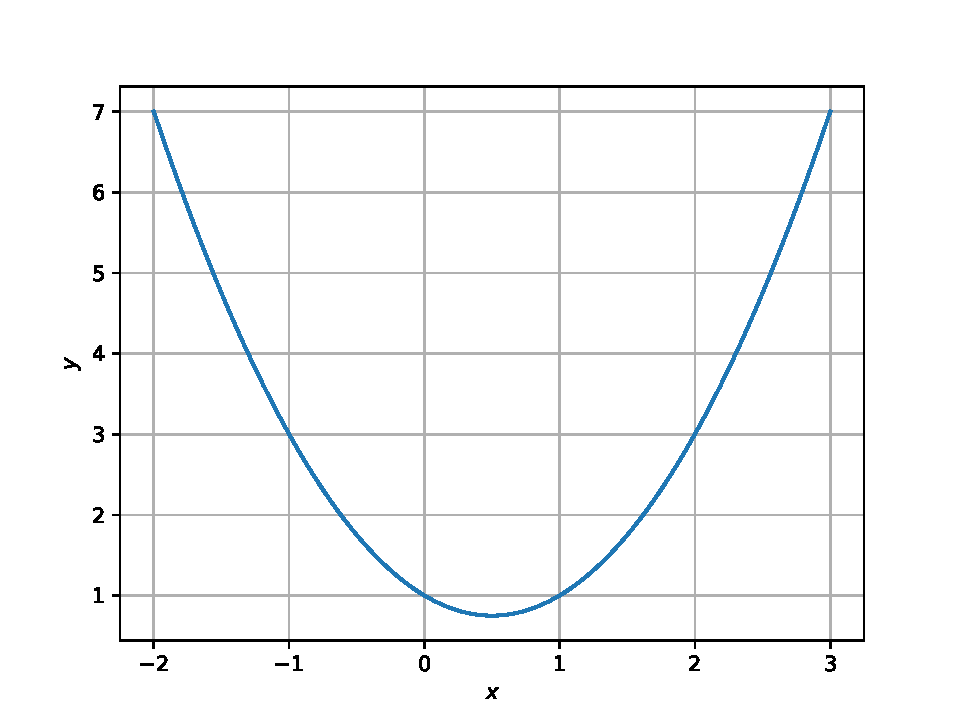
\includegraphics[width=\columnwidth]{./solutions/5/figs/conics/q20b.eps}
	\caption{}
	\label{fig:5.2.5_qtob}	
	\end{figure}
	
		
Here, sum of zeroes = D = 1\\
Product of zeroes = F =1\\
Substituing the values in \ref{eq:5.2.5_qtwenty},\\
\begin{multline}
\vec{x}^T\myvec{1&0\\0&0}\vec{x}  + \myvec{-1&-1}\vec{x} +1 = 0
\end{multline}
\begin{align}
\implies y = x^2 - x + 1 
\end{align}
Since the curve doesn't meet the x-axis, real roots don't exist for this parabola as represented in Fig. \ref{fig:5.2.5_qtob}	
		\item 0,$\sqrt{5}$
			\begin{figure}[!ht]
	\centering
	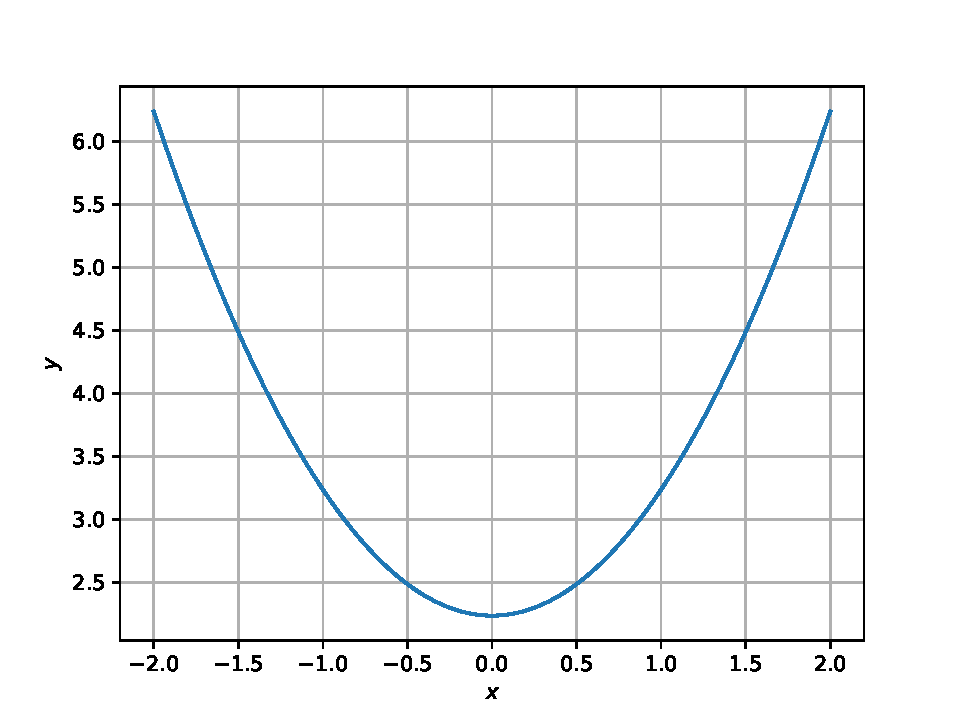
\includegraphics[width=\columnwidth]{./solutions/5/figs/conics/q20c.eps}
	\caption{}
	\label{fig:5.2.5_qtoc}	
	\end{figure}

		
Here, sum of zeroes = D = 0\\
Product of zeroes = F =$\sqrt{5}$\\
Substituing the values in \ref{eq:5.2.5_qtwenty},\\
\begin{multline}
\vec{x}^T\myvec{1&0\\0&0}\vec{x}  + \myvec{0&-1}\vec{x} + \sqrt{5} = 0
\end{multline}
\begin{align}
\implies y = x^2 + \sqrt{5}  
\end{align}
Since the curve doesn't meet the x-axis, real roots don't exist for this parabola as represented in Fig. \ref{fig:5.2.5_qtoc}	
		\item 4,1
	\begin{figure}[!ht]
	\centering
	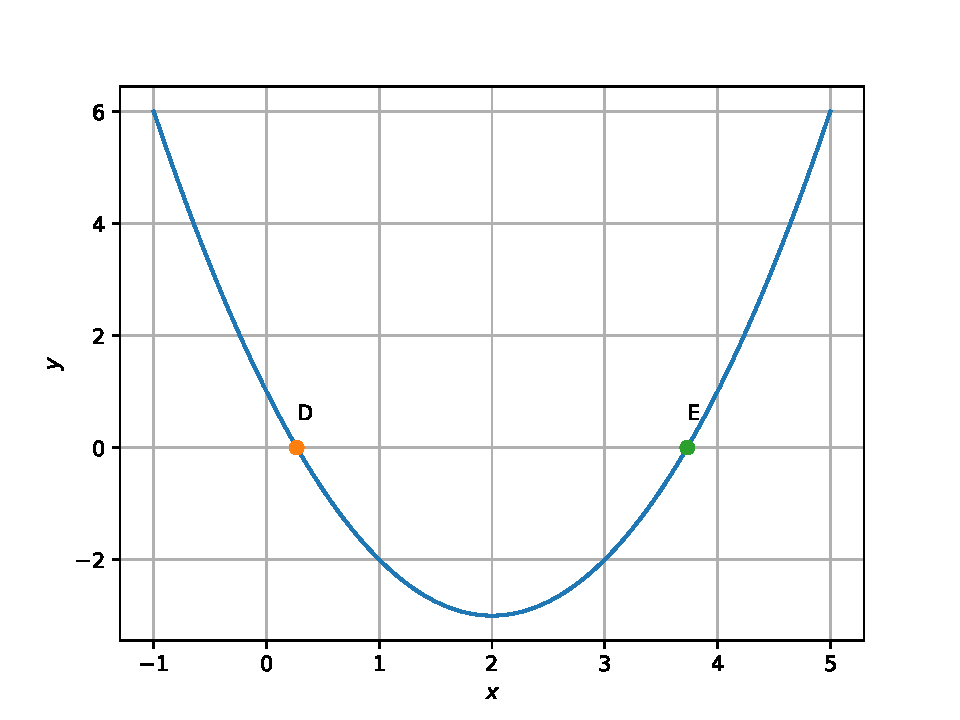
\includegraphics[width=\columnwidth]{./solutions/5/figs/conics/q20d.eps}
	\caption{}
	\label{fig:5.2.5_qtod}	
	\end{figure}
	
		 
Here, sum of zeroes = D = 4\\
Product of zeroes = F = 1\\
Substituing the values in \ref{eq:5.2.5_qtwenty},\\
\begin{multline}
\vec{x}^T\myvec{1&0\\0&0}\vec{x}  + \myvec{-4&-1}\vec{x} + 1 = 0
\end{multline}
\begin{align}
\implies y = x^2 - 4x + 1 
\end{align}
The roots are 3.73 and 0.26 as represented in Fig. \ref{fig:5.2.5_qtod}

		\item $\frac{1}{4}$,$\frac{1}{4}$
	\begin{figure}[!ht]
	\centering
	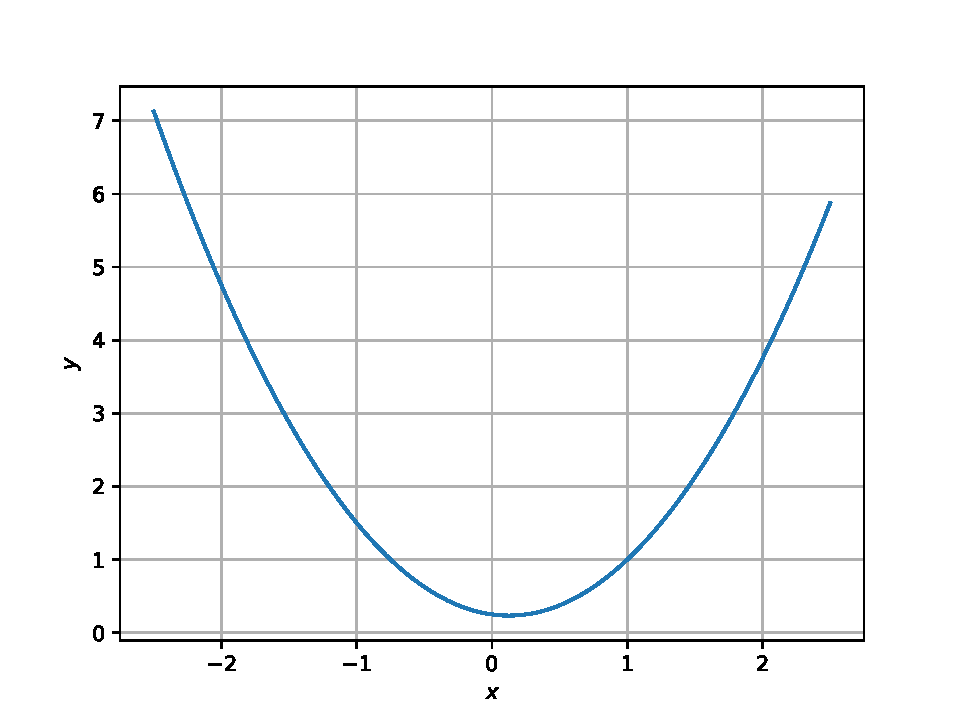
\includegraphics[width=\columnwidth]{./solutions/5/figs/conics/q20e.eps}
	\caption{}
	\label{fig:5.2.5_qtoe}	
	\end{figure}
		
 
Here, sum of zeroes = D = $\frac{1}{4}$\\
Product of zeroes = F = $\frac{1}{4}$\\
Substituing the values in \ref{eq:5.2.5_qtwenty},\\

\begin{multline}
\vec{x}^T\myvec{1&0\\0&0}\vec{x}  + \myvec{-\frac{1}{4}&-1}\vec{x} + \frac{1}{4} = 0
\end{multline}
\begin{align}
\implies y = x^2 - \frac{1}{4}x + \frac{1}{4} 
\end{align}
Since the curve doesn't meet the x-axis, real roots don't exist for this parabola as represented in Fig. \ref{fig:5.2.5_qtoe}	

		\item $\sqrt{2}$,$\frac{1}{3}$
	\begin{figure}[!ht]
	\centering
	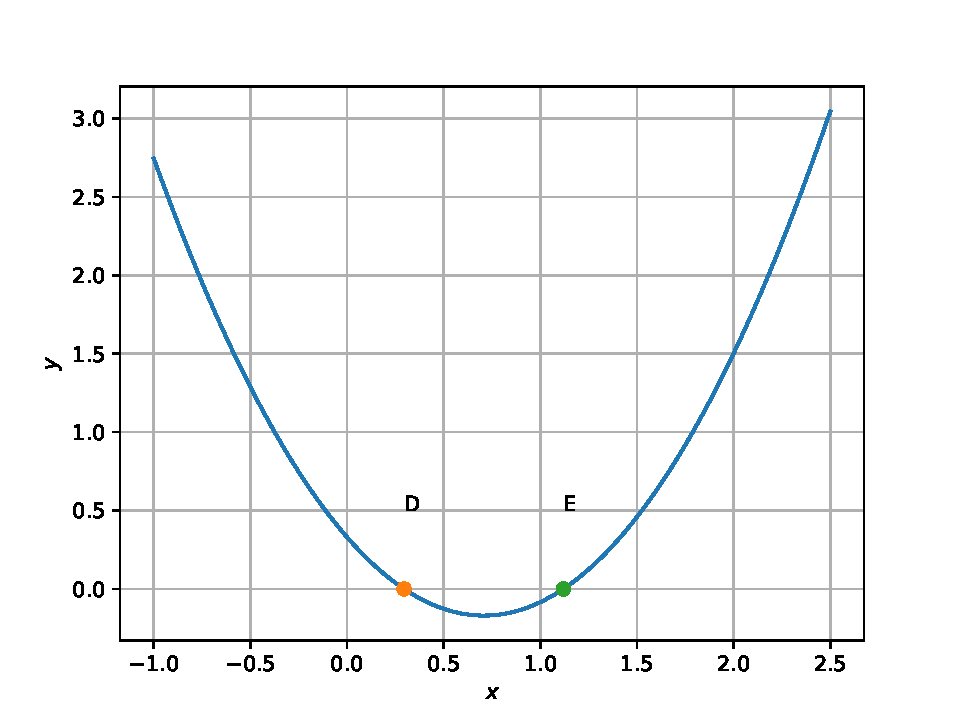
\includegraphics[width=\columnwidth]{./solutions/5/figs/conics/q20f.eps}
	\caption{}
	\label{fig:5.2.5_qtof}	
	\end{figure}

		

Here, sum of zeroes = D = $\sqrt{2}$\\
Product of zeroes = F = $\frac{1}{3}$\\
Substituing the values in \ref{eq:5.2.5_qtwenty},\\
\begin{multline}
\vec{x}^T\myvec{1&0\\0&0}\vec{x}  + \myvec{-\sqrt{2}&-1}\vec{x} + \frac{1}{3} = 0
\end{multline}
\begin{align}
\implies y = x^2 - \sqrt{2}x + \frac{1}{3}
\end{align}
The roots are 1.11 and 0.29 as represented in Fig. \ref{fig:5.2.5_qtof}
	\end{enumerate}

\item Find the roots of the following quadratic equations:
\begin{enumerate}
\item $x^2 – 3x – 10=0$
\item $2x^2+x-6=0$
\item $\sqrt{2}x^2 +7x+5\sqrt{2}  = 0$
\item $2x^2– x +\frac{1}{8} = 0 $
\item $100x^2 – 20x +1 = 0$
\end{enumerate}
\solution 
The given curve 
\begin{align}
	y =\frac{1}{x-1}
\end{align}
can be expressed as 
\begin{align}
	xy - y - 1 = 0 \label{eq:solutions/1/14/eq:hyperbola}
\end{align}
Hence, we have
\begin{align}
	\vec{V} = \frac{1}{2}\myvec{0 & 1 \\ 1 & 0}, 
	\vec{u} = \frac{1}{2}\myvec{0 \\-1},
	f = -1
\end{align}
Since $\mydet{\vec{V}} < 0$, the equation \eqref{eq:solutions/1/14/eq:hyperbola} represents hyperbola.
To find the values of $\lambda_1$ and $\lambda_2$, consider the characteristic equation,
\begin{align}
	\mydet{\lambda\vec{I} - \vec{V}} &= 0\\
	\implies \mydet{\myvec{\lambda & 0\\0 & \lambda} - \myvec{0 & \frac{1}{2} \\ \frac{1}{2} & 0}} &= 0\\
	\implies \mydet{ \lambda & \frac{-1}{2} \\ \frac{-1}{2} & \lambda} &= 0\\
	\implies \lambda_1 &= \frac{1}{2} , \lambda_2 = \frac{-1}{2}
\end{align}
In addition, given the slope -1, the direction and normal vectors are given by 
\begin{align}
	\vec{m} = \myvec{1 \\ -1} \\
	\vec{n} = \myvec{ 1 \\ 1}
\end{align}
The parameters of hyperbola are as follows:
\begin{align}
	\vec{c} &= -\vec{V}^{-1}\vec{u} \\
	&= -\myvec{0 & 2\\ 2 & 0}\myvec{0 \\ -\frac{1}{2}} \\
	&= \myvec{1 \\ 0}\\
	axes &= \begin{cases}
	\sqrt{\frac{\vec{u}^T\vec{V}^{-1}\vec{u} - f}{\lambda_1}} = \sqrt{2}\\
 \sqrt{\frac{f-\vec{u}^T\vec{V}^{-1}\vec{u}}{\lambda_2}} = \sqrt{2}
\end{cases}
\end{align}
which represents the standard hyperbola equation,
\begin{align}
	\frac{x^2}{2} - \frac{x^2}{2} = 1
\end{align}
The points of contact are given by 
\begin{align}
  \tiny{K} &=\pm \sqrt{\frac{\vec{u}^T\vec{V}^{-1}\vec{u} - f}{\vec{n}^T\vec{V}^{-1}\vec{n}}}
  = \pm \frac{1}{2}\\
  \vec{q} &= \vec{V}^{-1}(k\vec{n}-\vec{u})\\
  \vec{q_1} &= \myvec{0 & 2\\2 & 0} \sbrak{\frac{1}{2}\myvec{1 \\ 1} - \myvec{0\\ \frac{-1}{2}}}\\
  &= \myvec{2 \\ 1}\\
  \vec{q_2} &= \myvec{0 & 2\\2 & 0} \sbrak{\frac{-1}{2}\myvec{1 \\ 1} - \myvec{0\\ \frac{-1}{2}}}\\
  &= \myvec{0 \\ -1}
\end{align} 
$\therefore$ The tangents are given by
\begin{align}
	\myvec{1 & 1} \brak{\vec{x} - \myvec{2 \\ 1}} = 0 \\
	\myvec{1 & 1} \brak{\vec{x} - \myvec{0 \\ -1}} = 0
\end{align}
The desired equations of all lines having slope -1 that are tangents to the curve $\frac{1}{x-1}, x \neq 1$ are given by
\begin{align}
	\myvec{1 & 1}\vec{x} &= 3 \\
	\myvec{1 & 1}\vec{x} &= -1 
\end{align}
The above results are verified in the following figure.
\begin{figure}[h!] \label{eq:solutions/1/14/fig:tangents}
	\centering
	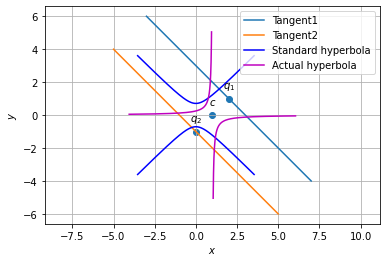
\includegraphics[width=\columnwidth]{./solutions/1/14/graph7.png}
	\caption{The standard and actual hyperbola.}
\end{figure}

\item Find the roots of the following quadratic equations
\begin{enumerate}
\item 	$2x^2-7x+3 = 0$
\item 	2$x^2+x-4 = 0$
\item 	$4x^2+4\sqrt{3}x+3 = 0$
\item 	2$x^2+x+4 = 0$
\end{enumerate}
\solution 
The given curve 
\begin{align}
	y =\frac{1}{x-1}
\end{align}
can be expressed as 
\begin{align}
	xy - y - 1 = 0 \label{eq:solutions/1/14/eq:hyperbola}
\end{align}
Hence, we have
\begin{align}
	\vec{V} = \frac{1}{2}\myvec{0 & 1 \\ 1 & 0}, 
	\vec{u} = \frac{1}{2}\myvec{0 \\-1},
	f = -1
\end{align}
Since $\mydet{\vec{V}} < 0$, the equation \eqref{eq:solutions/1/14/eq:hyperbola} represents hyperbola.
To find the values of $\lambda_1$ and $\lambda_2$, consider the characteristic equation,
\begin{align}
	\mydet{\lambda\vec{I} - \vec{V}} &= 0\\
	\implies \mydet{\myvec{\lambda & 0\\0 & \lambda} - \myvec{0 & \frac{1}{2} \\ \frac{1}{2} & 0}} &= 0\\
	\implies \mydet{ \lambda & \frac{-1}{2} \\ \frac{-1}{2} & \lambda} &= 0\\
	\implies \lambda_1 &= \frac{1}{2} , \lambda_2 = \frac{-1}{2}
\end{align}
In addition, given the slope -1, the direction and normal vectors are given by 
\begin{align}
	\vec{m} = \myvec{1 \\ -1} \\
	\vec{n} = \myvec{ 1 \\ 1}
\end{align}
The parameters of hyperbola are as follows:
\begin{align}
	\vec{c} &= -\vec{V}^{-1}\vec{u} \\
	&= -\myvec{0 & 2\\ 2 & 0}\myvec{0 \\ -\frac{1}{2}} \\
	&= \myvec{1 \\ 0}\\
	axes &= \begin{cases}
	\sqrt{\frac{\vec{u}^T\vec{V}^{-1}\vec{u} - f}{\lambda_1}} = \sqrt{2}\\
 \sqrt{\frac{f-\vec{u}^T\vec{V}^{-1}\vec{u}}{\lambda_2}} = \sqrt{2}
\end{cases}
\end{align}
which represents the standard hyperbola equation,
\begin{align}
	\frac{x^2}{2} - \frac{x^2}{2} = 1
\end{align}
The points of contact are given by 
\begin{align}
  \tiny{K} &=\pm \sqrt{\frac{\vec{u}^T\vec{V}^{-1}\vec{u} - f}{\vec{n}^T\vec{V}^{-1}\vec{n}}}
  = \pm \frac{1}{2}\\
  \vec{q} &= \vec{V}^{-1}(k\vec{n}-\vec{u})\\
  \vec{q_1} &= \myvec{0 & 2\\2 & 0} \sbrak{\frac{1}{2}\myvec{1 \\ 1} - \myvec{0\\ \frac{-1}{2}}}\\
  &= \myvec{2 \\ 1}\\
  \vec{q_2} &= \myvec{0 & 2\\2 & 0} \sbrak{\frac{-1}{2}\myvec{1 \\ 1} - \myvec{0\\ \frac{-1}{2}}}\\
  &= \myvec{0 \\ -1}
\end{align} 
$\therefore$ The tangents are given by
\begin{align}
	\myvec{1 & 1} \brak{\vec{x} - \myvec{2 \\ 1}} = 0 \\
	\myvec{1 & 1} \brak{\vec{x} - \myvec{0 \\ -1}} = 0
\end{align}
The desired equations of all lines having slope -1 that are tangents to the curve $\frac{1}{x-1}, x \neq 1$ are given by
\begin{align}
	\myvec{1 & 1}\vec{x} &= 3 \\
	\myvec{1 & 1}\vec{x} &= -1 
\end{align}
The above results are verified in the following figure.
\begin{figure}[h!] \label{eq:solutions/1/14/fig:tangents}
	\centering
	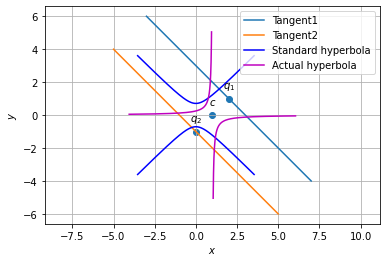
\includegraphics[width=\columnwidth]{./solutions/1/14/graph7.png}
	\caption{The standard and actual hyperbola.}
\end{figure}

\item Factorise $6x^2+ 17x + 5$.
\\
\solution 

The given polynomial can be expressed as:
\begin{align}
\vec{x}^T \myvec{6 & 0\\0 & 0}\vec{x}+ \myvec{17 & 0}\vec{x}+5=0
\end{align}
Substituting y=0 in the above equation,
\begin{align}
 6x^2+17x+5 &=0\\
\implies x&=\frac{-1}3{},\frac{-5}{2}\\
\therefore (3x+1)(2x+5) &=6x^2+17x+5
\end{align}
%
which is verified in Fig.     \ref{quadform/16/Fig:Graph Of $x^2+7x+10 &=$.}

\begin{figure}[ht!]
    \centering
    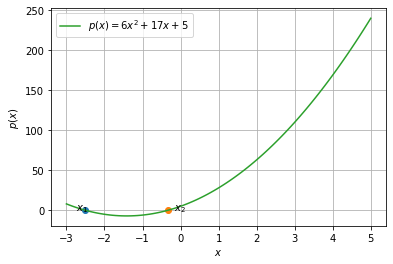
\includegraphics[width=\columnwidth]{solutions/su2021/2/16/Graph.png}
    \caption{Graph of $6x^2+17x+5$.}
    \label{quadform/16/Fig:Graph Of $x^2+7x+10 &=$.}
\end{figure}



\item Find the zeroes of the polynomial $x^2-3$ and verify the relationship between the zeroes and the coefficients.
\\
\solution 
From the given information, for 
\begin{align}
\Vec{A} &=  \myvec{2 \\ 5 } , \Vec{B} =  \myvec{-3 \\ 6},
\vec{m} &= \vec{A}-\vec{B}
\\
& = \myvec{5 \\ -1}
\\
\implies \vec{n}& = \myvec{5 \\ -1}
\end{align}
Let 
\begin{align}
    \vec{P} = \myvec{-3\\5}
\end{align}
The equation of the desired line is then obtained as
\begin{align}
\label{linform/15/eq:line_norm_vec}
\vec{n}^T\brak{\vec{x}-\vec{P}} &= 0
\\
\implies \myvec{5 & -1} \vec{x} &= -20
\end{align}
and plotted in Fig. \ref{linform/15/fig: Perpendicular Bisector}	
\begin{figure}[!ht]
\centering
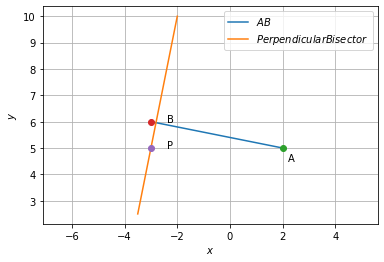
\includegraphics[width=\columnwidth]{solutions/su2021/2/15/download (6).png}
\caption{Perpendicular Bisector}
\label{linform/15/fig: Perpendicular Bisector}	
\end{figure}

\item Find the discriminant of the quadratic equation $2x^2-4x+3 = 0$
hence find the nature of its roots.
\\
\solution
From the given information, for 
\begin{align}
\Vec{A} &=  \myvec{2 \\ 5 } , \Vec{B} =  \myvec{-3 \\ 6},
\vec{m} &= \vec{A}-\vec{B}
\\
& = \myvec{5 \\ -1}
\\
\implies \vec{n}& = \myvec{5 \\ -1}
\end{align}
Let 
\begin{align}
    \vec{P} = \myvec{-3\\5}
\end{align}
The equation of the desired line is then obtained as
\begin{align}
\label{linform/15/eq:line_norm_vec}
\vec{n}^T\brak{\vec{x}-\vec{P}} &= 0
\\
\implies \myvec{5 & -1} \vec{x} &= -20
\end{align}
and plotted in Fig. \ref{linform/15/fig: Perpendicular Bisector}	
\begin{figure}[!ht]
\centering
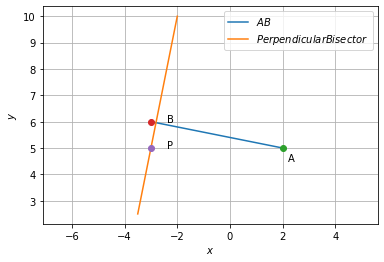
\includegraphics[width=\columnwidth]{solutions/su2021/2/15/download (6).png}
\caption{Perpendicular Bisector}
\label{linform/15/fig: Perpendicular Bisector}	
\end{figure}

\item Find the discriminant of the quadratic equation $3x^2-2x+\frac{1}{3} = 0$
hence find the nature of its roots.
\\
\solution

The given equation can be expressed as
\begin{align}
\vec{x}^T \myvec{3 & 0\\0 & 0}\vec{x}+ 2\myvec{-1 \\ \frac{-1}{2}}\vec{x}+\frac{1}{3}=0
\end{align}
with
\begin{align}
\vec{V} = \myvec{3 & 0 \\ 0 & 0},\vec{u}=\myvec{-1 \\ \frac{-1}{2}},f=\frac{1}{3}
\end{align}
Using eigenvalue decomposition,
\begin{align}
\vec{D} = \myvec{0 & 0\\0 & 3} ,\vec{P}=\myvec{0 & 1\\1 & 0}
\end{align}
Thus,
\begin{align}
\myvec{\vec{u}^T + \eta\vec{p_1}^T \\ \vec{V}}\vec{c} &= \myvec{-f \\ \eta\vec{p_1}-\vec{u}} 
\\
\implies \myvec{-1 & -1 \\ 3 & 0 \\ 0 & 0}\vec{c} &= \myvec{\frac{-1}{3}\\ 1 \\ 0} \\
\implies  \myvec{-1 & -1 \\ 3 & 0}\vec{c} &= \myvec{\frac{-1}{3}\\ 1}
\\
\implies \vec{c} &= \myvec{\frac{1}{3}\\0}
\end{align}
$\because$
\begin{align}
\vec{p_1}^T\vec{c} &= \myvec{0 & 1}\myvec{\frac{1}{3}\\0}
\\
&= 0
\\
\vec{p_2}^T\vec{V}\vec{p_2} &= \myvec{1 & 0}\myvec{3 & 0\\0& 0}\myvec{1 \\ 0}
\\
&= 3,
\end{align}
$\because$
\begin{align}
(\vec{p_1}^T\vec{c})(\vec{p_2}^T\vec{V}\vec{p_2}) = 0
\end{align}
Thus, the given equation has  real and equal roots which can be verified from Fig. \ref{quadforms/2/25/Roots of}.  
%
\begin{figure}[!ht]
\centering
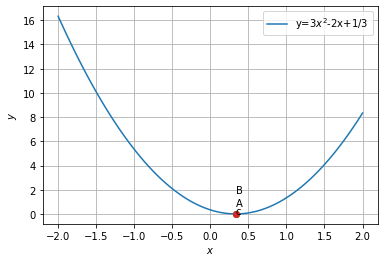
\includegraphics[width=\columnwidth]{solutions/su2021/2/25/download (3).png}
\caption{Roots of $3x^2 -2x + 1/3 = 0$ }
\label{quadforms/2/25/Roots of}
\end{figure}






\item Find the equation of all lines having slope 2 and being tangent to the curve
\begin{align}
y + \frac{2}{x-3} = 0
\end{align}
%
\\
\solution
\documentclass[journal,12pt,twocolumn]{IEEEtran}
\usepackage{graphicx}
\graphicspath{{./figs/}}{}
\usepackage{amsmath,amssymb,amsfonts,amsthm}
\newcommand{\myvec}[1]{\ensuremath{\begin{pmatrix}#1\end{pmatrix}}}

\let\vec\mathbf

\title{
Matrix-Conics
}
\author{Kukunuri Sampath Govardhan}
\begin{document}
\maketitle
\tableofcontents
\bigskip

\section{Problem Statement}
\begin{flushleft}
In an Ellipse, the distance between its foci is 6 and minor axis is 8. Then find its Eccentricity.\\
\end{flushleft}
\section{Construction}
\begin{figure}[h]
    \centering
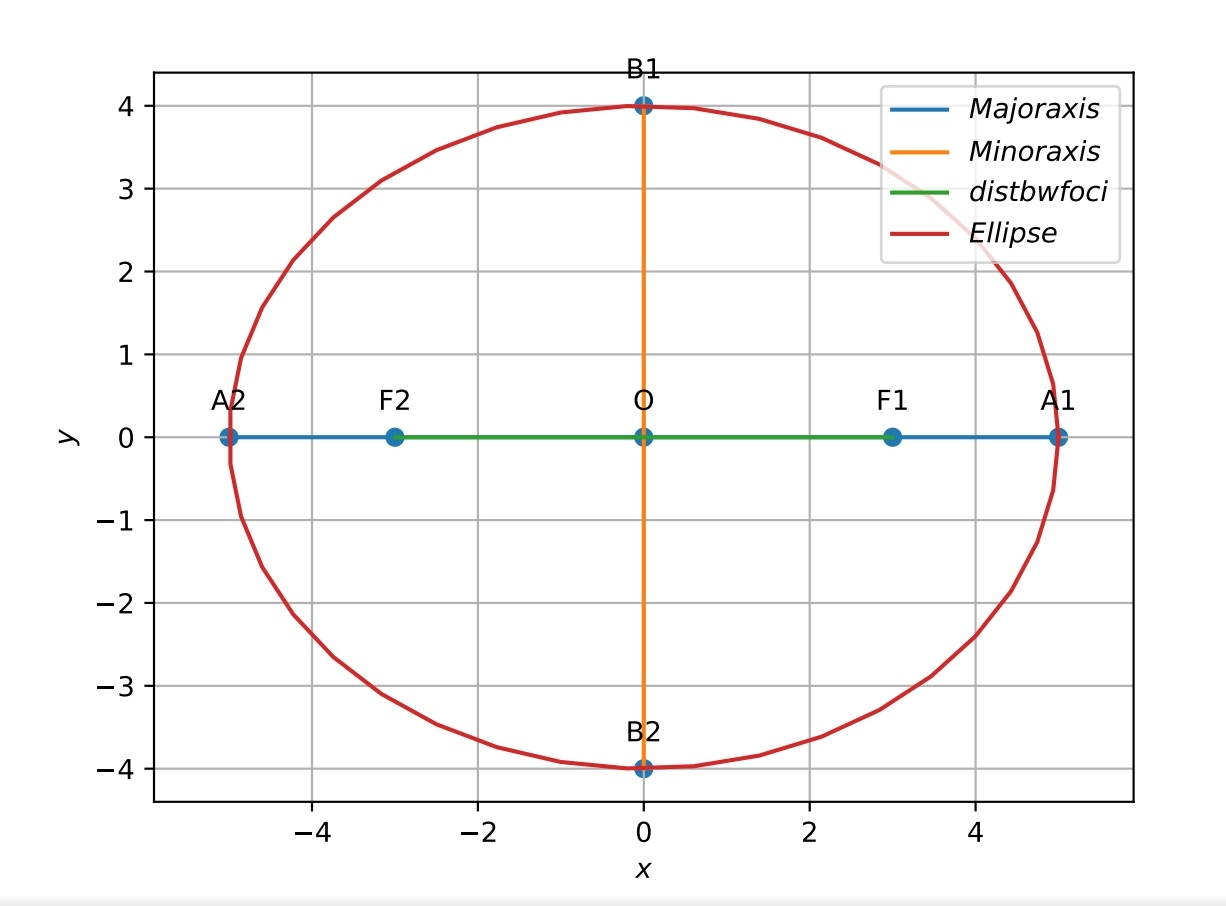
\includegraphics[width=\columnwidth]{figs/assign6.png}
    \caption{Ellipse}
    \label{fig:my_label}
\end{figure}
\begin{table}[h]
    \centering
    \begin{tabular}{|c|c|c|}
       \hline
       \textbf{Symbol}&\textbf{Value}&\textbf{Description}  \\
       \hline
            ${||\vec{F_1} - \vec{F_2}||}$ & 6 & Distance between foci\\
        \hline
            ${||\vec{B_1} - \vec{B_2}||}$ & 8 & Length of Minor axis\\
        \hline
        $\vec{e_1}$ & \myvec{1 \\ 0} & Standard Basis Vector \\
        \hline
        e & & Eccentricity \\
            \hline
    \end{tabular}
    \caption{Parameters}
    \label{tab:my_label}
\end{table}
\vspace{2cm}
\section{Solution}
The length of minor axis in ellipse is\\
\begin{equation}
        ||\vec{B_1} - \vec{B_2}|| = 2\sqrt{|\frac{f_0}{\lambda_2}|}\label{eq-1}
\end{equation}
Therefore,\\
\begin{center}
	8 = $2\sqrt{|\frac{f_0}{\lambda_2}|}$
\end{center}
Yielding,\\
\\
\begin{equation}
\frac{f_0}{\lambda_2} = 16 \label{eq-2}\\
\end{equation}
\\
The focal points \\
\begin{equation}
        \vec{F_1} =
        \frac{\frac{1}{e\sqrt{1 - e^2}}e^2\sqrt{\frac{\lambda_2}{f_0}}\vec{e_1}}{\frac{\lambda_2}{f_0}}
\end{equation}
\begin{equation}
        \vec{F_2} = -
        \frac{\frac{1}{e\sqrt{1 - e^2}}e^2\sqrt{\frac{\lambda_2}{f_0}}\vec{e_1}}{\frac{\lambda_2}{f_0}}
\end{equation}
\begin{center}
$||\vec{F_1} - \vec{F_2}|| = 2\frac{\frac{1}{e\sqrt{1 - e^2}}e^2\sqrt{\frac{\lambda_2}{f_0}}||\vec{e_1}||}{\frac{\lambda_2}{f_0}}$ \\
\vspace{0.3cm}
$6 = \frac{\frac{1}{\sqrt{1 - e^2}}e\sqrt{\frac{\lambda_2}{f_0}}}{\frac{\lambda_2}{f_0}}$
\end{center}
Substuting $\frac{\lambda_2}{f_0}$ from eq-2, \\
\begin{equation}
       6 = 2\frac{e}{\sqrt{1 - e^2}}\frac{1}{4}\frac{16}{1}
\end{equation}
 Yielding,   \\
 \begin{center}
	 $e = \frac{3}{5}$ 
 \end{center}
 Therefore,\\
\\
\begin{center}
$\boldsymbol{Eccentricity, e = \frac{3}{5}}$ 
\end{center}
\end{document}




\item Find the point at which the tangent to the curve $y = \sqrt{4x-3}-1$ has its 
slope $\frac{2}{3}$.
%
\\
\solution
Given curve,
\begin{align}
y = \sqrt{4x-3}-1\label{quadform/42/2.0.1}\\
\implies (y+1)^2 =4x-3\\
\implies y^2-4x+2y+4 =0
\end{align}
which has the vector parameters
\begin{align}
\vec{V}&=\myvec{0 & 0 \\ 0 & 1},\vec{u}=\myvec{-2 & 1 }, \vec{f} = 4 
\end{align}
\begin{align}
|\vec{V}| = 0
\end{align}
$\therefore $ the given curve \eqref{quadform/42/2.0.1} is parabola. In standard form,
\begin{align}
\vec{P} =\vec{I}\implies \vec{p_1} = \myvec{1 \\ 0}
\end{align}
Since the slope of the tangents is $\frac{2}{3}$, the direction and normal vectors are
\begin{align}
\vec{m} &= \myvec{1\\\frac{2}{3}}= \myvec{3\\2},\vec{n} = \myvec{2\\-3}\\
\text{and }
\kappa &= \frac{\vec{p_1^T}\vec{u}}{\vec{p_1^T}\vec{n}} = -1
\end{align}
$\therefore$ Point of contact for the tangent is
\begin{align}
  \myvec{\vec{u}+\kappa \vec{n^T}\\\vec{V} }\vec{q} &= \myvec{\vec{-f}\\\kappa \vec{n} -\vec{u}}\\
  \implies\myvec{-4 & 4\\0 & 0 \\0 & 1} \vec{q}&= \myvec{-4\\0\\2}\\
  \implies \vec{q}&=\myvec{3\\2}
\end{align}
%$\therefore $ Point of contact for tangent of given curve is
% \begin{align}
% \vec{q }= \myvec{3\\2}
% \end{align}
which is verified in Fig.     \ref{quadform/42/fig:Tangent to parabola.}
%
\begin{figure}[ht]
    \centering
    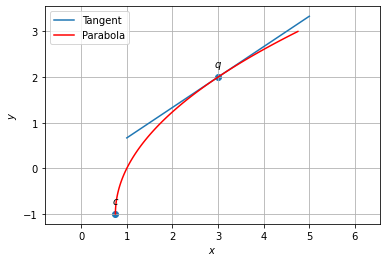
\includegraphics[width=\columnwidth]{solutions/su2021/2/42/PARABOLA.png}
    \caption{Tangent to Parabola.}
    \label{quadform/42/fig:Tangent to parabola.}
\end{figure}    



\item Find the equation of the normal to the curve $x^2= 4y$
which passes through the point \myvec{1\\ 2}.
%
\solution
The given curve can be expressed as 
\begin{align}
 x^2-4y &=0 \label{quadform/45/2.0.2}
 \\
%\vec{x}^T\vec{V}\vec{x}+2\vec{u}^T\vec{x}+f=0\\
\implies \vec{V}=\myvec{1 & 0 \\ 0 & 0},\vec{u}=\myvec{0 \\ -2 }, \vec{f} = 0 
\end{align}
$\because$
\begin{align}
 \abs{\vec{V}} &= 0
\end{align}
the given curve \eqref{quadform/45/2.0.2} represents a parabola.
The eigenvalues are given by 
\begin{align}
\lambda_1 = 0 , \lambda_2 = 1
\end{align}
with corresponding eigenvectors
\begin{align}
\myvec{1 & 0 \\ 0 & 0}\vec{x} &=0 \implies \vec{p_1} = \myvec{0 \\ 1}
\\
\myvec{0 & 0 \\ 0 & -1}\vec{x} &=0 \implies \vec{p_2} = \myvec{1 \\ 0}
\end{align}
To find the vertex of the parabola ,
\begin{align} \myvec{\vec{u^T}+\kappa\vec{p_1^T}\\\vec{V} }\vec{c} &= \myvec{\vec{-f}\\\kappa \vec{p_1} -\vec{u}}
\\
\text{where, }  \kappa = \vec{u^T}\vec{p_1} = -2
\\
\implies\myvec{0 & -4\\1 & 0 \\0 & 0} \vec{c}&= \myvec{0\\0\\0} \label{quadform/45/eq:b}
\end{align}
from the above it can be observed that,
\begin{align}    
   \vec{c} &= \myvec{0 \\ 0}
\end{align}
Now to evalute the direction vector m,
\begin{align}
\vec{m}^T(\vec{V}\vec{q} + \vec{u}) &=0
\\
\implies \vec{m}^T\brak{\myvec{1 & 0 \\ 0 & 0}\myvec{1 \\ 2} + \myvec{0 \\ -2}} &=0
\\
\implies \vec{m}^T\myvec{1 \\ -2} &=0
\\
\implies \vec{m} = \myvec{-2 \\ -1}
\end{align}
The normal is obtained as 
\begin{align}
\vec{m}^T(\vec{x} - \vec{q}) &=0 
\\
\myvec{-2 & -1}\brak{\vec{x}-\myvec{1 \\ 2}} &= 0
\\
\myvec{-2 & -1}\vec{x}+ 4 &= 0 
\end{align}
%
The above results are verified in Fig.     \ref{quadform/45/fig:Normal to parabola.}.
\begin{figure}[ht]
    \centering
    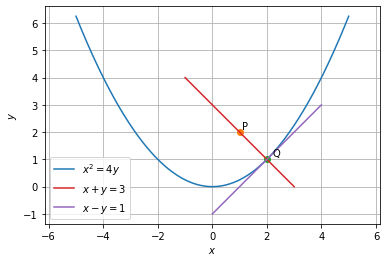
\includegraphics[width=\columnwidth]{solutions/su2021/2/45/FIGURE4.png}
    \caption{Normal to Parabola.}
    \label{quadform/45/fig:Normal to parabola.}
\end{figure}    


%
\item Find the intervals in which the function 
\begin{align}
f(x)  = x^2-4x+6
\end{align}
%
is 
\begin{enumerate}
\item increasing
\item decreasing.
\end{enumerate}
%
\solution
From the given information, for 
\begin{align}
\Vec{A} &=  \myvec{2 \\ 5 } , \Vec{B} =  \myvec{-3 \\ 6},
\vec{m} &= \vec{A}-\vec{B}
\\
& = \myvec{5 \\ -1}
\\
\implies \vec{n}& = \myvec{5 \\ -1}
\end{align}
Let 
\begin{align}
    \vec{P} = \myvec{-3\\5}
\end{align}
The equation of the desired line is then obtained as
\begin{align}
\label{linform/15/eq:line_norm_vec}
\vec{n}^T\brak{\vec{x}-\vec{P}} &= 0
\\
\implies \myvec{5 & -1} \vec{x} &= -20
\end{align}
and plotted in Fig. \ref{linform/15/fig: Perpendicular Bisector}	
\begin{figure}[!ht]
\centering
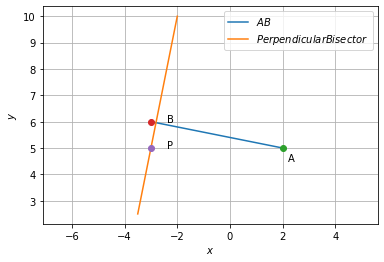
\includegraphics[width=\columnwidth]{solutions/su2021/2/15/download (6).png}
\caption{Perpendicular Bisector}
\label{linform/15/fig: Perpendicular Bisector}	
\end{figure}

\item Find the equation of the parabola with focus \myvec{2\\0} and directrix $\myvec{1 & 0}\vec{x} = -2$.\item Find the equation of the parabola with vertex at \myvec{0\\ 0} and focus at \myvec{0\\ 2}.
\\
\solution
The equation of the plane is given by 
\begin{align}
\vec{n}^T\brak{\vec{x}-\vec{A}} &= 0
\\
\implies \myvec{1 & 1 & -1}{\vec{x}} &= \myvec{1 & 1 & -1}{\myvec{1\\0\\-2}}
\\
\text{or, }\myvec{1 & 1 & -1}{\vec{x}} &= 3
\end{align}
and plotted in Fig. \ref{linform/35/1/Plot of the plane}.

\begin{figure}[ht]
\centering
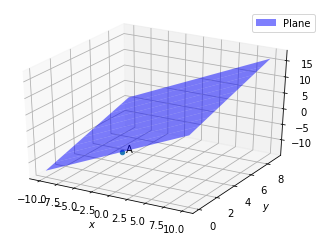
\includegraphics[width=\columnwidth]{solutions/su2021/2/35/1/Plane_plot1.PNG}
\caption{Plot of the plane}
\label{linform/35/1/Plot of the plane}
\end{figure}


%
\item Find the equation of the ellipse, with major axis along the x-axis and passing through the points \myvec{4\\ 3} and \myvec{– 1\\4}.
\\
\solution
Let 
\begin{align}
\vec{p} = \myvec{4\\3} , \vec{q} = \myvec{– 1\\4}
\end{align}
%
In general, the equation of the ellipse passing through $\vec{p}, \vec{q}$ can be expressed as
\begin{align}
\brak{\vec{x}-\vec{c}}^{\top}\vec{D}\brak{\vec{x}-\vec{c}}=1\label{quadforms/37/eq:14}
\end{align}
where the center $\vec{c}=\myvec{\beta\\0}$ and 
 $\vec{D}$ is a diagonal matrix.
$\because \vec{p}, \vec{q}$ satisfy \eqref{quadforms/37/eq:14},
\begin{align}
\label{quadforms/37/eq:ellipse_std_ab}
(\vec{p}-\vec{c})^{\top}\vec{D}(\vec{p}-\vec{c}) &= 1,
\\
(\vec{q}-\vec{c})^{\top}\vec{D}(\vec{q}-\vec{c}) &= 1,
\end{align}
which can be simplified as 
\begin{align}
    2\brak{\vec{p}-\vec{q}}^{\top}\vec{D}\vec{c}=\vec{p}^{\top}\vec{D}\vec{p}-\vec{q}^{\top}\vec{D}\vec{q}
\end{align}
Using the identity, 
\begin{multline}
    \brak{\vec{p}-\vec{q}}^{\top}\vec{D}(\vec{p}+\vec{q})
   =\vec{p}^{\top}\vec{D}\vec{p}-\vec{q}^{\top}\vec{D}\vec{q}
\end{multline}
in the above, 
\begin{multline}
    2\brak{\vec{p}-\vec{q}}^{\top}\vec{D}\vec{c}  = \brak{\vec{p}-\vec{q}}^{\top}\vec{D}(\vec{p}+\vec{q})
    \\
    \implies \brak{\vec{p}-\vec{q}}^{\top}\vec{D}\brak{2\vec{c}-\brak{\vec{p}+\vec{q}}} = 0
\end{multline}
Thus, $\vec{c}$ can be expressed in parametric form as 
\begin{align}
    \vec{c}=\frac{1}{2}\sbrak{\vec{p}+\vec{q}+ k\vec{D}^{-1}\vec{m}}
    \label{quadform/37/centre}
    \end{align}
    where 
\begin{align}
    (\vec{p}-\vec{q})^{\top}\vec{m}=0
    \label{quadform/37/dir}
\end{align}
and $k$ is a constant.  Substituting numerical values in     \eqref{quadform/37/dir},
\begin{align}
    \vec{p}-\vec{q} &= \myvec{5 \\ -1}
    \implies \vec{m} = \myvec{1 \\ 5}
\end{align}
Also, 
\begin{align}
    \vec{p}+\vec{q} &= \myvec{3 \\ 7}
\end{align}
which, upon substitution in     \eqref{quadform/37/centre} yields 
\begin{align}
 \myvec{\beta\\0}=\frac{1}{2}\sbrak{\myvec{3\\7}+k\myvec{\frac{1}{\lambda_1} & 0 \\ 0 & \frac{1}{\lambda_2}}\myvec{1\\5}}
\end{align}
From the given information, the $X-$axis is the major axis.  Hence, 
\begin{align}
    \frac{\lambda_2}{\lambda_1}>1
    \implies \frac{2\beta-3}{\frac{-7}{5}}>1\\
    \text{or, } \beta<0.8
\end{align}
%
The possible ellipses satisfying the above condition are plotted in Fig. \ref{quadforms/37/fig:ellipses}.	
\begin{figure}[!ht]
\centering
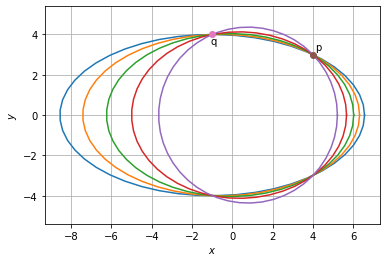
\includegraphics[width=\columnwidth]{solutions/su2021/2/37/figure5_1.png}
\caption{Ellipses passing through the two points with X axis as major axis}
\label{quadforms/37/fig:ellipses}	
\end{figure}
%

\item Find the coordinates of the foci and the vertices, the eccentricity,the length of the latus rectum of the hyperbolas
\begin{enumerate}
\item 
$
\vec{x}^T\myvec{\frac{1}{9} & 0 \\ 0 & -\frac{1}{16}}\vec{x} = 1
$
\item 
$
\vec{x}^T\myvec{1 & 0 \\ 0 & -16}\vec{x} = 16
$
\end{enumerate}
\solution
\begin{enumerate}
    \item 
    From the given information, for 
\begin{align}
\Vec{A} &=  \myvec{2 \\ 5 } , \Vec{B} =  \myvec{-3 \\ 6},
\vec{m} &= \vec{A}-\vec{B}
\\
& = \myvec{5 \\ -1}
\\
\implies \vec{n}& = \myvec{5 \\ -1}
\end{align}
Let 
\begin{align}
    \vec{P} = \myvec{-3\\5}
\end{align}
The equation of the desired line is then obtained as
\begin{align}
\label{linform/15/eq:line_norm_vec}
\vec{n}^T\brak{\vec{x}-\vec{P}} &= 0
\\
\implies \myvec{5 & -1} \vec{x} &= -20
\end{align}
and plotted in Fig. \ref{linform/15/fig: Perpendicular Bisector}	
\begin{figure}[!ht]
\centering
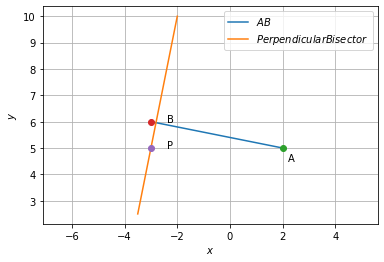
\includegraphics[width=\columnwidth]{solutions/su2021/2/15/download (6).png}
\caption{Perpendicular Bisector}
\label{linform/15/fig: Perpendicular Bisector}	
\end{figure}


From the given equation, 
\begin{align}
    \vec{V} = \myvec{1 & 0 \\ 0 & -16}
    \\
    \vec{u}^{\top}\vec{V}^{-1}\vec{u}-f = 16
    \\
    \vec{c} = -\vec{V}^{-1}\vec{u}=\myvec{0 \\ 0}
    \\
    \lambda_1 = 1 , \lambda_2 = -16
\end{align}
Axes of hyperbola are given by
\begin{align}
    \sqrt{\frac{\vec{u}^{\top}\vec{V}^{-1}\vec{u}-f}{\lambda_1}} = 4\\ \sqrt{\frac{f-\vec{u}^{\top}\vec{V}^{-1}\vec{u}}{\lambda_2}} = 1
\end{align}
and the vertices are
\begin{align}
    \pm\myvec{4 \\ 0} 
\end{align}
Coordinates of the foci are given by,
\begin{align}
  \vec{F} =\pm\brak{\sqrt{\frac{(\vec{u}^T\vec{V}^{-1}\vec{u}-f)(\lambda_2-\lambda_1)}{\lambda_1\lambda_2}}}\vec{p_1} \label{quadform/2/38/b/eq:1}
\end{align}
where, $\vec{p_1} = \myvec{1 \\ 0}$ since the equation of hyperbola is in standard form.
Substituting the values in \eqref{quadform/2/38/b/eq:1} we have,
\begin{align}
    \vec{F} = \pm\myvec{\sqrt{17} \\ 0}.
\end{align}
Eccentricity of the hyperbola is given by,
\begin{align}
   e &= \frac{\sqrt{\frac{(\vec{u}^{\top}\vec{V}^{-1}\vec{u})(\lambda_2-\lambda_1)}{\lambda_1\lambda_2}}}{\sqrt{\frac{\vec{u}^{\top}\vec{V}^{-1}\vec{u}-f}{\lambda_1}}} \label{quadform/2/38/b/eq:2}
   &= \frac{\sqrt{17}}{4}.
\end{align}
upon substituting from  \eqref{quadform/2/38/b/eq:2}.
Length of the latus rectum is given by,
\begin{align}
    l &= \frac{2\brak{{\sqrt{\frac{f-\vec{u}^{\top}\vec{V}^{-1}\vec{u}}{\lambda_2}}}}^2}{\sqrt{\frac{\vec{u}^{\top}\vec{V}^{-1}\vec{u}-f}{\lambda_1}}} \label{quadform/2/38/b/eq:3}
    &= \frac{1}{2}
\end{align}
upon substituting the values in \eqref{quadform/2/38/b/eq:3}.
The above results are verified in Fig. \ref{quadform/2/38/b/Plot of standard hyperbola}.

\begin{figure}[ht]
\centering
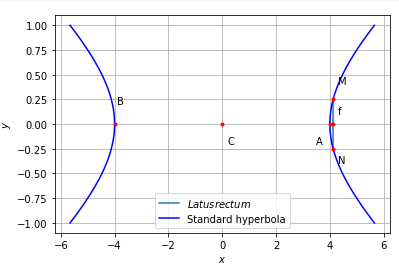
\includegraphics[width=\columnwidth]{solutions/su2021/2/38/b/hyperbola.PNG}
\caption{Plot of standard hyperbola}
\label{quadform/2/38/b/Plot of standard hyperbola}
\end{figure}


\end{enumerate}
%
\item Find the slope of the tangent to the curve $y = \frac{x-1}{x-2}, x\ne 2$ at $x = 10$.
\\
\solution 
The given curve,
% \begin{align}
% y&=\frac{{x-1}}{{x-2}} 
% \end{align}
 can be expressed as,
\begin{align}
yx-2y-x+1 =0
\label{quadform/75/2.0.1}
\end{align}
yielding
\begin{align}
\vec{V}&=\myvec{\frac{1}{2} & 0 \\ 0 & \frac{1}{2}},\vec{V}^{-1}=\myvec{0&2\\2&0}\vec{u}=\myvec{-\frac{1}{2}\\-1},
f =1 \label{quadform/75/2.0.3}
\end{align}
\begin{align}
\because  |\vec{V}| < 0
\end{align}
 \eqref{quadform/75/2.0.1} is a hyperbola.
Let the slope of tangent be $r$. Then the  direction vector and normal vector of tangent to \eqref{quadform/75/2.0.1} are
\begin{align}
    \vec{m}&= \myvec{1\\r},\vec{n}=\myvec{r\\-1} \label{quadform/75/2.0.5}\\
\kappa=&\pm \sqrt{\frac{\vec{u^T}\vec{V}^{-1}\vec{u}-\vec{f}}{\vec{n^T}\vec{V}^{-1}\vec{n}}}\\
&=\sqrt{\frac{-1}{4r}} \label{quadform/75/2.0.8}
\end{align}
For hyperbola, the point of contact for the tangent is
\begin{align}
\vec{q}&=\vec{V}^{-1}(\kappa\vec{n}-\vec{u})\label{quadform/75/2.0.6}\\
\implies \vec{V}\vec{q}+\vec{u}&=\kappa\vec{n}\\
\implies \myvec{\frac{1}{16}\\4}&=\kappa\vec{n} \quad ( \text{ From } \quad \eqref{quadform/75/2.0.3})\\
\implies \myvec{\frac{1}{16}\\4}&=\sqrt{\frac{-1}{4r}}\myvec{r\\-1}\\
\implies \myvec{\frac{1}{16}\\4}&=\myvec{r\sqrt{\frac{-1}{4r}}\\-\sqrt{\frac{-1}{4r}}}\\
\implies -\sqrt{\frac{-1}{4r}}&=4\\
\implies r &= -\frac{1}{64}
\end{align}
which is the desired slope. Fig.     \ref{quadform/75/fig:Tangent to HYPERBOLA.} verifies this result.
\begin{figure}[!ht]
    \centering
    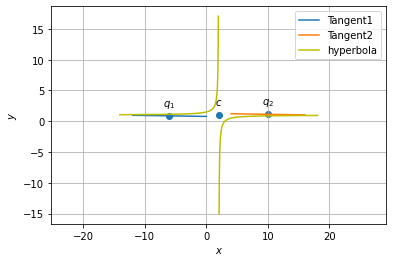
\includegraphics[width=\columnwidth]{solutions/su2021/2/75/HYPERBOLA.png}
    \caption{Tangent to HYPERBOLA.}
    \label{quadform/75/fig:Tangent to HYPERBOLA.}
\end{figure}  



\item Find the equation of all lines having slope 2 which are tangents to the curve $\frac{1}
{x - 3} , x \ne 3$.
%
\\
\solution

Given curve  
\begin{align}
    y &= \frac{1}{x-3} , x \neq 3 \label{quadform/78/giveneq}
    \\
    \implies xy - 3y - 1 &= 0
\end{align}

$\therefore$
\begin{align}
    \vec{V} &= \frac{1}{2}\myvec{0 & 1 \\ 1 & 0}
    \\
    \vec{u} &= \frac{-3}{2}\myvec{0 \\ 1}
    \\
    f &= -1
\end{align}

$\because$
\begin{align}
    \abs{\vec{V}} &= \frac{-1}{4}
    \\
    \implies \abs{\vec{V}} &< 0
\end{align}
$\therefore$ \eqref{quadform/78/giveneq} represents a hyperbola .
Now,the characteristic equation of $\vec{V}$ is 
\begin{align}
    \abs{\vec{V} - \lambda\vec{I}} = \mydet{-\lambda & \frac{1}{2} \\ \frac{1}{2} & -\lambda} &= 0
    \\
    \implies \lambda^2 - \frac{1}{4} &= 0
\end{align}
$\therefore$ Eigen values are 
\begin{align}
    \lambda_1 = \frac{1}{2} , \lambda_2 = \frac{-1}{2}
\end{align}
Eigen vector $\vec{p}$ is 
\begin{align}
    \vec{V}\vec{p} &= \lambda\vec{p}
    \\
    \implies (\vec{V} - \lambda\vec{I})\vec{p} &= 0
\end{align}
Eigen vector $\vec{p}_1$ corressponding to $\lambda_1$ can be obtained as
\begin{align}
    (\vec{V} - \lambda_1\vec{I}) &= \myvec{\frac{-1}{2} & \frac{1}{2} \\ \frac{1}{2} & \frac{-1}{2}}\xleftrightarrow[R_1 \leftarrow -2R_1]{R_2 = R_1 + R_2}\myvec{1 & -1 \\ 0 & 0}
    \\
    \implies \vec{p_1} &= \frac{1}{\sqrt{2}}\myvec{1 \\ 1}
\end{align}
Similarly,
\begin{align}
    \vec{p_2} &= \frac{1}{\sqrt{2}}\myvec{-1 \\ 1}
\end{align}
$\therefore$
\begin{align}
    \vec{P} &= \myvec{\vec{p_1} & \vec{p_2}} = \frac{1}{\sqrt{2}}\myvec{1 & -1 \\ 1 & 1}
    \\
    \vec{D} &= \myvec{\lambda_1 & 0 \\ 0 & \lambda_2} = \myvec{\frac{1}{2} & 0 \\ 0 & \frac{-1}{2}}
\end{align}
Now,
\begin{align}
    \vec{c} &= -\vec{V}^{-1}\vec{u} 
    \\
    &= -\myvec{0 & 2 \\2 & 0}\myvec{0 \\ \frac{-3}{2}}
    \\
    &= \myvec{3 \\ 0}
\end{align}
and
\begin{align}
    \sqrt{\frac{ \vec{u}^T\vec{V}^{-1}\vec{u} - f}{\lambda_1}} &= \sqrt{2}
    \\
    \sqrt{ \frac{f- \vec{u}^T\vec{V}^{-1}\vec{u}}{\lambda_2}} &= \sqrt{2}
\end{align}
$\therefore$ Equation of standard hyperbola can be expressed as 
\begin{align}
    \frac{x^2}{2} - \frac{y^2}{2} &= 1
\end{align}
Now,direction vector of tangent with slope = 2 is
\begin{align}
    \vec{m} &= \myvec{1 \\ m} = \myvec{1 \\ 2}
\end{align}
and,normal vector of same tangent is 
\begin{align}
    \vec{m}^T\vec{n} &= 0
    \\
    \implies \vec{n} &= \myvec{2 \\ -1} 
\end{align}
Now,
\begin{align}
    \kappa &= \pm \sqrt{\frac{\vec{u}^T\vec{V}^{-1}\vec{u}-f}{\vec{n}^T\vec{V}^{-1}\vec{n}}}
    \\
    &= \pm \sqrt{\frac{1}{-8}}
\end{align}
$\therefore$ Real value of $\kappa$ does not exist and hence points of contacts of tangent $\vec{q_1},\vec{q_2}$ also does not exist.
\\
Hence,there exists no tangent to the curve having slope = 2.  The hyperbola is plotted in Fig. \ref{quadform/78/fig:hyperbola}.	
%
\begin{figure}[!ht]
\centering
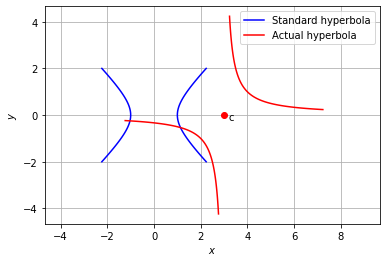
\includegraphics[width=\columnwidth]{solutions/su2021/2/78/Figure8.png}
\caption{Standard and actual hyperbola}
\label{quadform/78/fig:hyperbola}	
\end{figure}



\item Find points on the curve 
$
\vec{x}^T\myvec{\frac{1}{9} & 0 \\ 0 & \frac{1}{16}}\vec{x} = 1
$
%
at which tangents are
\begin{enumerate}
\item  parallel to x-axis
\item  parallel to y-axis.
\end{enumerate}
%
\solution

Given curve,
\begin{align}
\vec{x}^T\myvec{\frac{1}{9} & 0 \\ 0 & \frac{1}{16}}\vec{x} = 1 \label{quad/79/2.0.1}
\end{align}
where,
\begin{align}
\vec{V}&=\myvec{\frac{1}{9} & 0 \\ 0 & \frac{1}{16}},\vec{V}^{-1}=\myvec{9&0\\0&16}\vec{u}=0, f = -1 
\end{align}
\begin{align}
\because |\vec{V}| > 0
\end{align}
given curve \eqref{quad/79/2.0.1} is ellipse.
For an ellipse, the point of contact for the tangent is
\begin{align}
\vec{q}&=\vec{V}^{-1}(\kappa\vec{n}-\vec{u})\\
&=\vec{V}^{-1}\kappa\vec{n}\quad\quad\quad(\because \vec{u}=0). \label{quad/79/2.0.5}
\end{align}
where,
\begin{align}
\kappa=&\pm \sqrt{\frac{\vec{u^T}\vec{V}^{-1}\vec{u}-f}{\vec{n^T}\vec{V}^{-1}\vec{n}}}\\
      =&\pm \sqrt{\frac{-f}{\vec{n^T}\vec{V}^{-1}\vec{n}}}\label{quad/79/2.0.7}\quad \quad\quad(\because \vec{u}=0)
\end{align}
\begin{enumerate}
\item For the tangents  parallel to x-axis, then direction and normal vectors are,
\begin{align}
\vec{m_1} = \myvec{1\\0},\vec{n_1} = \myvec{0\\1},
\kappa_1 &=\pm \sqrt{\frac{-f}{\vec{n_1^T}\vec{V}^{-1}\vec{n_1}}} \\
 &=\pm\frac{1}{4}
\end{align}
$\therefore$ By Substituting $\kappa_1,\vec{n_1},\vec{V}^{-1}$ in \eqref{quad/79/2.0.5}
\begin{align}
\vec{q}&=\vec{V}^{-1}\kappa_1\vec{n_1} \\
&=\myvec{0\\\pm4}
\end{align}
% $\therefore$ Point of contact for tangents of ellipse are,
% \begin{align}
%   \vec{q_1}=\myvec{0\\4},\vec{q_2}=\myvec{0\\-4}
% \end{align}
\item For the tangents  parallel to the y-axis, the direction and normal vectors are
\begin{align}
\vec{m_2} = \myvec{0\\1},\vec{n_2} = \myvec{1\\0},
\kappa_2 &=\pm \sqrt{\frac{-f}{\vec{n_2^T}\vec{V}^{-1}\vec{n_2}}} \\
 &=\pm\frac{1}{3}
\end{align}
$\therefore$ substituting $\kappa_2,\vec{n_2},\vec{V}^{-1}$ in \eqref{quad/79/2.0.5}
\begin{align}
\vec{q}&=\vec{V}^{-1}\kappa_2\vec{n_2} \\
&=\myvec{0\\\pm3}
\end{align}
% $\therefore$ Point of contact for tangents of ellipse are,
% \begin{align}
%   \vec{q_3}=\myvec{3\\0},\vec{q_4}=\myvec{-3\\0}
% \end{align}
\end{enumerate}
The above results are verified in Fig.     \ref{quad/79/fig:Tangent to ELLIPSE.}
%
\begin{figure}[!ht]
    \centering
    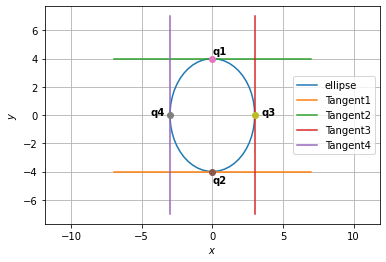
\includegraphics[width=\columnwidth]{solutions/su2021/2/79/ELLIPSE.png}
    \caption{Tangents to ELLIPSE.}
    \label{quad/79/fig:Tangent to ELLIPSE.}
\end{figure}  


\item Find the equation of the tangent to the curve $y = \sqrt{3x - 2}$ which is parallel to the line $\myvec{4 & -2}\vec{x}+ 5 =0$ .
%
\solution
The given equation can be expressed as 
\begin{align}
    \vec{x}^{\top}\myvec{0&0 \\ 0&1}\vec{x}+\myvec{-3&0}\vec{x}+2=0 \label{quadform/82/eq:giveneq}
\end{align}
and 
\begin{align}
\therefore \vec{u}=\myvec{\frac{-3}{2} \\ 0}
\\
\vec{V} =\myvec{0&0 \\ 0&1}
\\
\implies {\mydet{\vec{V}}}=0
\end{align}
Thus the curve is a parabola with eigenvalues 
\begin{align}
 \lambda= 0,1
\end{align}
The corresponding  eigenvectors are 
\begin{align}
    \myvec{0&0 \\ 0&1}\vec{x} = 0\implies \vec{p_{1}}= \myvec{1 \\ 0}
    \\
    \myvec{-1&0 \\ 0&0}\vec{x} = \vec{x}\implies \vec{p_{2}}= \myvec{0 \\ 1}
\end{align}
and 
\begin{align}
    \vec{V} = \vec{P}\vec{D}\vec{P}^{\top}\label{quadform/82/eq:eqn1}
\end{align}
where 
\begin{align}
 \vec{P} = \myvec{\vec{p_{1}} & \vec{p_{2}}} = \myvec{1&0 \\ 0&1}
 \\
 \vec{D}=\myvec{\lambda_{1}&0 \\ 0&\lambda_{2}} = \myvec{0&0 \\ 0&1}
\end{align}
Since the given parallel line equation  is 
\begin{align}
 \myvec{4&-2}\vec{x} + 5 = 0, \label{quadform/82/eq:eqn2}
\end{align}
%Now the tangent to the parabola is parallel to the line equation \eqref{quadform/82/eq:eqn2},
the normal vector $\vec{n}$ and the direction vector $\vec{m}$ of the tangent to the parabola are given by 
\begin{align}
    \vec{n}=\myvec{4 \\ -2} \label{quadform/82/eq:eqn5}
    \\
    \vec{m}=\myvec{-2 \\ -4}
\end{align}
The  point of contact for the parabola is given by,
\begin{align}
    \myvec{\vec{u}+\kappa \vec{n}^{\top} \\ \vec{V} }\vec{q} 
    = \myvec{\vec{-f}\\\kappa \vec{n} -\vec{u}}
    \\
  \implies \kappa =\frac{\vec{p_{1}}^{\top}\vec{u}}{\vec{p_{1}}^{\top}\vec{n}}
    =\frac{\myvec{1&0}\myvec{\frac{-3}{2} \\ 0}}{\myvec{1&0}\myvec{4 \\ 2}}
    =\frac{-3}{8}
    \end{align}
and 
\begin{align}
    \myvec{-3&\frac{3}{4} \\ 0&0 \\ 0&1} \vec{q}&= \myvec{-2 \\ 0 \\ \frac{3}{4}}
\end{align}
% Now solving for $\vec{q}$ by removing the zero row and representing as augmented matrix and then converting it to echelon form.
% \begin{align}
%     \myvec{-3&\frac{3}{4}&-2 \\ 0&1&\frac{3}{4}}\xleftrightarrow{R_1\rightarrow \brak{\frac{-1}{3}}R_1} \myvec{1&\frac{-1}{4}&\frac{2}{3} \\ 0&1&\frac{3}{4}}
%     \\
%     \myvec{1&\frac{-1}{4}&\frac{2}{3} \\ 0&1&\frac{3}{4}}\xleftrightarrow{R_1\rightarrow R_1+\frac{1}{4}R_2}\myvec{1&0&\frac{41}{48} \\ 0&1&\frac{3}{4}} \label{quadform/82/eq:eqn3}
% \end{align}
%Hence from the \eqref{quadform/82/eq:eqn3} we get the point of contact to be 
yielding 
\begin{align}
    \vec{q}=\myvec{\frac{41}{48} \\ \frac{3}{4}}
\end{align}
The desired equation of the line is 
%Now $\vec{q}$ is the point on the tangent.Hence the equation of the line can be expressed as 
\begin{align}
    \mathbf{n}^{\top}(\mathbf{x}-\mathbf{q}) &= 0\label{quadform/82/eq:eqn6}
    \\
% \end{align}
% where,
% \begin{align}
% \vec{n}^{\top}\vec{q}
%     =\myvec{4&-2}\myvec{\frac{41}{48} \\ \frac{3}{4}} 
%     \\
%     = \frac{23}{12} \label{quadform/82/eq:eqn4}
% \end{align}
% Hence the equation of the tangent to the curve \eqref{quadform/82/eq:giveneq} parallel to the line \eqref{quadform/82/eq:eqn2} is given by substituting the value of $\vec{n}^{\top}\vec{q}$ and $\vec{n}$ from \eqref{quadform/82/eq:eqn4} and \eqref{quadform/82/eq:eqn5} respectively to the equation \eqref{quadform/82/eq:eqn6} 
% \begin{align}
\implies     \myvec{4&-2}\vec{x}&=\frac{23}{12} \label{quadform/82/eq:eqn7}
\end{align}
which is verified in Fig. \ref{quadform/82/Plot of curve and the lines}.
% Hence \eqref{quadform/82/eq:eqn7} is the equation of the tangent.
% The plot of the figure is given below
%
\begin{figure}[ht]
\centering
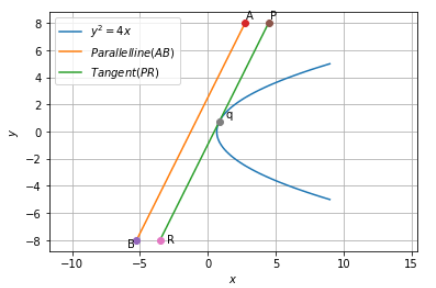
\includegraphics[width=\columnwidth]{solutions/su2021/2/82/Parabola.PNG}
\caption{Plot of curve and the lines}
\label{quadform/82/Plot of curve and the lines}
\end{figure}
%
\item AOBA is the part of the ellipse 
$
\vec{x}^T\myvec{9 & 0 \\ 0 & 1}\vec{x} = 36
$
in the first quadrant such that $OA = 2$ and $OB = 6$. Find the area between the arc $AB$ and the chord $AB$.
\\
\solution
Given ellipse is 
\begin{align}
    \vec{x}^T\myvec{9 & 0 \\ 0 & 1}\vec{x} = 36 
\end{align}

On comparing it with standard form
\begin{align}
    \vec{c} &= \myvec{0 \\ 0}
    \\
    \vec{D} &= \myvec{9 & 0 \\ 0 & 1}
    \\
    \vec{u}^T\vec{V}^{-1}\vec{u} - f &= 36
    \\
    \lambda_1 &= 9 
    \\
    \lambda_2 &= 1
\end{align}

$\therefore$  Semi major and minor axes of ellipse are
\begin{align}
    a &= \sqrt{\frac{ \vec{u}^T\vec{V}^{-1}\vec{u} - f}{\lambda_2}} = \sqrt{\frac{36}{1}} = 6
    \\
    b &= \sqrt{\frac{ \vec{u}^T\vec{V}^{-1}\vec{u} - f}{\lambda_1}} = \sqrt{\frac{36}{9}} = 2
\end{align}
$\therefore$ Equation of ellipse can be written as
\begin{align}
    \frac{x^2}{a^2} + \frac{y^2}{b^2} &= 1
    \\
    \implies \frac{x^2}{4} + \frac{y^2}{36} &= 1
\end{align}

Now,area of ellipse is given by
\begin{align}
    A &= \pi ab
    \\
    \implies A &= 12\pi
\end{align}

$\therefore$ Area of a quadrant of ellipse is given by
\begin{align}
    A_1 &= A/4 = 3\pi
\end{align}

Now,from Fig. \ref{quadform/2/99/fig:ellipse} , $AOBA$ is a right angled triangle whose area is given by 
\begin{align}
    A_2 &= \frac{1}{2}ab = 6
\end{align}

$\therefore$ Area between arc $AB$ and chord $AB$ is given by
\begin{align}
    A_3 &= A_1 - A_2 = 3\pi -6
\end{align}


\begin{figure}[!ht]
\centering
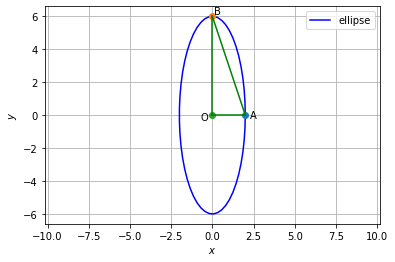
\includegraphics[width=\columnwidth]{solutions/su2021/2/99/Figure7.png}
\caption{Ellipse $\frac{x^2}{4} + \frac{y^2}{36} = 1$}
\label{quadform/2/99/fig:ellipse}	
\end{figure}



\item Find the area enclosed by the parabola $4y = 3x^2$ and the line $\myvec{-3 & 2}\vec{x} = 12$.
%
\\
\solution
\begin{lemma}
The points of intersection of \textbf{Line} $L:\vec{x}=\vec{q}+\mu\vec{m}$ with \textbf{parabola},are given by:
\begin{align}
\vec{x}_i = \vec{q}+\mu_i\vec{m}
\end{align}
%
where,
\begin{multline}
\mu_i = \frac{1}
{
\vec{m}^T\vec{V}\vec{m}
}
\lbrak{-\vec{m}^T\brak{\vec{V}\vec{q}+\vec{u}}}
\\
\pm
{\small
\rbrak{\sqrt{
\sbrak{
\vec{m}^T\brak{\vec{V}\vec{q}+\vec{u}}
}^2
-
\brak
{
\vec{q}^T\vec{V}\vec{q} + 2\vec{u}^T\vec{q} +f
}
\brak{\vec{m}^T\vec{V}\vec{m}}
}
}
}\label{quadform/2/105/eq:mu_i}
\end{multline}
\end{lemma}
 The matrix parameters of the parabola are
\begin{align}
\vec{V}=\myvec{1&0\\0&0},\vec{u}=\myvec{0\\-\frac{2}{3}},f=0 \label{quadform/2/105/eq:v}
\end{align}
with eigen parameters 
\begin{align}
\lambda_1 &= 0 , \lambda_2 = 1
\\
\vec{p_1} &= \myvec{0 \\ 1},
\vec{p_2} = \myvec{1 \\ 0}
\end{align}
The vertex of the parabola can be expressed as
\begin{align} \myvec{\vec{u^T}+\eta\vec{p_1^T}\\\vec{V} }\vec{c} &= \myvec{\vec{-f}\\\eta \vec{p_1} -\vec{u}}
\\
\text{where, }  \eta = \vec{u^T}\vec{p_1} = \frac{-2}{3}
\\
\implies\myvec{0 & \frac{-4}{3}\\1 & 0 \\0 & 0} \vec{c}&= \myvec{0\\0\\0}
\\
\text{or, }
   \vec{c} &= \myvec{0 \\ 0}
\end{align}
From  \eqref{quadform/2/105/eq:mu_i},
\begin{align}
\mu_i &= \frac{1}{4}
\brak{10}
\pm{6}
\\
\implies \mu_1 &= 1, \mu_2 =4
\end{align}
The given line is
\begin{align} 
\myvec{-3&2}\vec{x}&=12
\end{align}
 In parametric form, the given  line can be written as:
\begin{align} 
L: \vec{x}&=\vec{q}+\mu\vec{m}
\\
\implies \vec{x}&=\myvec{-4\\0}+\mu\myvec{2\\3} \label{quadform/2/105/eq:q}
\end{align}
Substitutuing $\mu_1$ and $\mu_2$ in \eqref{quadform/2/105/eq:q},the points of intersection
\begin{align}
 \vec{K}= \myvec{-2\\3},  
\vec{L}&= \myvec{4\\12}
\end{align}

\begin{enumerate}
  \item Thus, from Fig. \ref{quadform/2/105/Plot of the Parabola and line} the area enclosed by parabola and line can be given as
\begin{align}
   A&= \text{Area under line} - \text{Area under parabola}
     \\
   A&= Ar(KLMNK)-Ar(KCLMCNK)
    \\
    A&= A_1 -A_2 \label{quadform/2/105/eqAREA}
    \end{align}
\item Area under the line 2y=3x+12 i.e, $A_1$-
\begin{align}
  A_1&= \int_{-2}^{4} y dx
    \\
    A_1&= \frac{1}{2}\int_{-2}^{4} \brak{3x+12} dx
    \end{align}
    \begin{align}
    A_1= \frac{3}{2}\int_{-2}^{4} x+\frac{1}{2}\int_{-2}^{4}12 dx
    \end{align}
    \begin{align}
    A_1&= \frac{3}{4}\brak{4^2-2^2} +\frac{12}{2}\brak{4+2}
   \\
    A_1&= \frac{3}{4}\brak{12} +\frac{12}{2}\brak{6}
    \\
    A_1&= 9 +36
    \\
    A_1 &=45 \text{ units} \label{quadform/2/105/eqB}
\end{align}
\item Area under the parabola that is $A_2$-
\begin{align}
    A_2&= \int_{-2}^{4} y dx
    \\
    A_2&= \int_{-2}^{4} \frac{3}{4} x^2 dx
    \\
    A_2&= \frac{3}{4} \int_{-2}^{4}  x^2 dx
    \\
    A_2&= \frac{3}{4\times3} \brak{4^3-\brak{-2}^3}
    \\
    A_2&= \frac{1}{4} \brak{64 +8}
    \\
    A_2&= \frac{72}{4} 
    \\
    A_2&= 18 \text{ units} \label{quadform/2/105/eqC}
\end{align}
\item Putting \eqref{quadform/2/105/eqB} and \eqref{quadform/2/105/eqC} in \eqref{quadform/2/105/eqAREA} we get required area A as:
\begin{align}
 A &= A_1 -A_2 
 \\
 A &= 45-18
 \\
 A &= 27 \text{ units}
\end{align}
%
\end{enumerate}
\begin{figure}[ht]
\centering
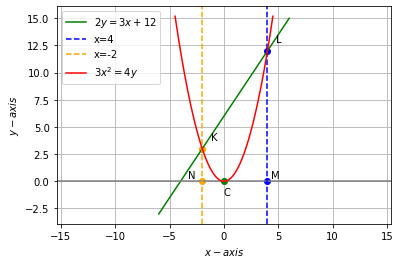
\includegraphics[width=\columnwidth]{solutions/su2021/2/105/LINE AND PARABOLA.png}
\caption{Plot of the parabola and line}
\label{quadform/2/105/Plot of the Parabola and line}
\end{figure}


%\item Verify whether the following are zeroes of the polynomial, indicated against them. (i) p(x) = 3x + 1, x =
%\begin{enumerate}
%
%\item $ p(x) = x^2-1, x = 1, -1$
%\item $ p(x) = 5x -\pi, x = \frac{4}{5}$
%\item $ p(x) = \brak{x+1} \brak{x-2}, x = -1,2$
%\item $ p(x) = x^2, x = 0$.
%\item $ p(x) = 3x^2-1, x = -\frac{1}{\sqrt{3}}, \frac{2}{\sqrt{3}}$.
%

%\end{enumerate}
